\renewcommand{\thechapter}{4}
\chapter{Denoising Theory and Implementation}
\label{ch:DenoisingTheory}

We have shown in section~\ref{sec:DetectorBackgrounds} that if it is possible to improve the energy resolution of EXO-200 then backgrounds, particularly from $^{232}$Th and $^{137}$Xe, can be reduced.  The energy resolution of EXO-200 is limited by its scintillation energy resolution, so any attempt to improve the energy resolution should focus on improved extraction of APD pulse magnitudes.  In this chapter we present a new technique for extracting optimal scintillation energy measurements based on an improved model of the pulses and noise on APD waveforms.  The estimator derived in this chapter will be optimal partly due to its ability to operate in the presence of noise; we will therefore describe it throughout as a ``denoising'' technique, though at no point are denoised waveforms produced.

We begin with a general overview in section~\ref{sec:WhatIsDenoising} of what qualitative methods of noise reduction a denoising technique may hope to apply and why they are necessary for our APDs.  Notational conventions and some crucial input parameters will be listed in section~\ref{sec:DenoisingNotationSetup}.  Section~\ref{sec:DescriptionOfPhotonNoise} presents a detailed physics model of the fluctuations in observed pulse magnitude, and section~\ref{sec:BridgePhotonsPulses} will connect that physics model to observable output of the APD channels.  The optimal energy estimator is presented in section~\ref{sec:DerivationOfEstimator} with a derivation.  Sections~\ref{sec:MatrixFormulationOfDenoising}-\ref{sec:DenoisingComputationalConsiderations} translate the optimal energy estimator into a usable form and describe the computational steps needed to apply it to data.  Differences between the optimal version of denoising presented in this chapter and the version used for the present physics analysis are shown in section~\ref{sec:DenoisingInPractice}.  We finish in section~\ref{sec:FutureDenoisingExtensions} by identifying some extensions to the denoising technique presented here which may prove interesting for future analyses.

\section{What is Denoising?}\label{sec:WhatIsDenoising}

Before the investigations described in this work, scintillation energy was not measured from individual APD channels.  Instead, two summed waveforms were constructed: a sum of all waveforms from APDs on the North plane, and a sum of all waveforms from APDs on the South plane.  This simplified the construction of a position-dependent correction function, or lightmap.  (For more details on why this is so, see section~\ref{ch:Lightmap}.  \textcolor{red}{UPDATE WITH A REAL SECTION REFERENCE WHEN I HAVE ONE.})  However, when we sum waveforms together we discard information; this section will show that the information which is thrown away is in fact critical to improving our scintillation energy measurements.

\begin{figure}
\begin{center}
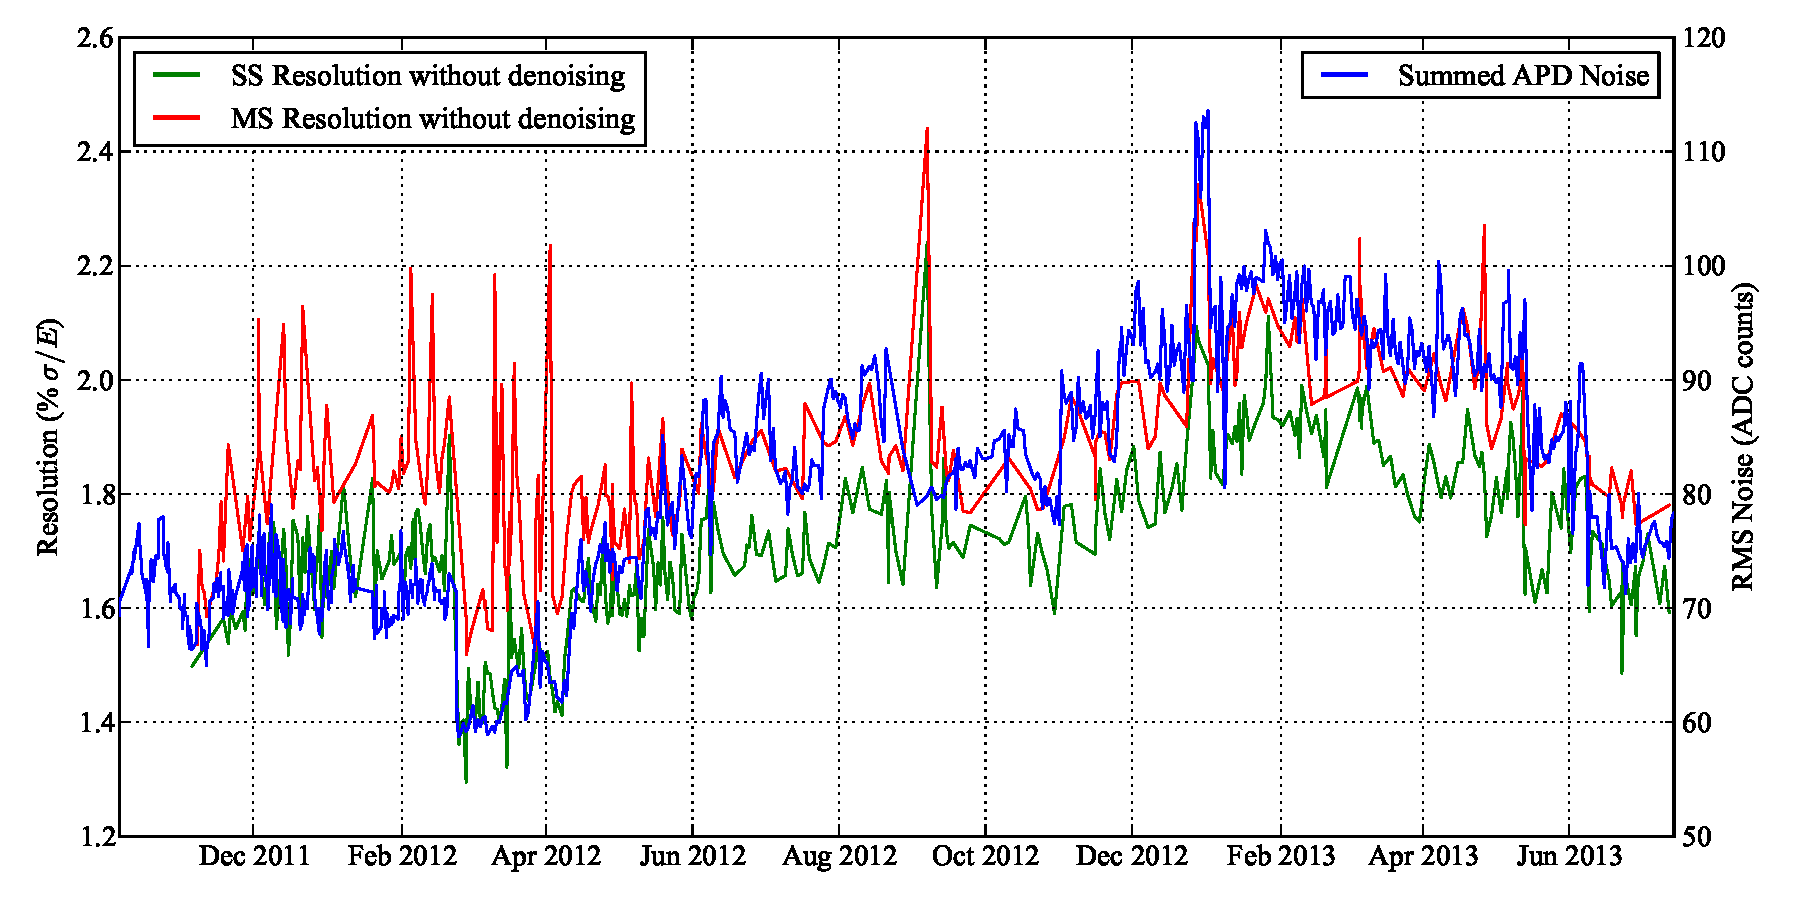
\includegraphics[keepaspectratio=true,width=\textwidth]{ResolutionAPDNoiseComparison.pdf}
\end{center}
\renewcommand{\baselinestretch}{1}
\small\normalsize
\begin{quote}
\caption{Detector energy resolution (without denoising) is strongly correlated with noise observed on the APDs.  Noise data provided by Josiah Walton.}
\label{fig:ResolutionAPDNoiseComparison}
\end{quote}
\end{figure}
\renewcommand{\baselinestretch}{2}
\small\normalsize

Energy resolution is a critical factor in the strength of the EXO-200 experiment.  Figure~\ref{fig:ResolutionAPDNoiseComparison} shows the energy resolution trend which was observed before denoising was developed.  We can see that there was a long period of worsening resolution from March 2012 to February 2013, when the single-site energy resolution changed from 1.4\% to 1.9\% $\sigma/E$ at our $Q$-value, followed by a period of improvement to 1.6\% in July 2013.  There has always been interest in ways to improve the energy resolution, but the upward trend gave greater urgency to understand the observed fluctuations, reverse them, and find a way to counter the effect in offline analysis for existing data.

A search began for environmental changes which could be correlated to the worsening energy resolution.  In addition to the energy resolution trend, figure~\ref{fig:ResolutionAPDNoiseComparison} overlays a trend of the root-mean-square noise on the sum of APD waveforms, and we can immediately see that the overall energy resolution is closely tied to electronic noise on the summed APD channels.

\begin{figure}
\begin{center}
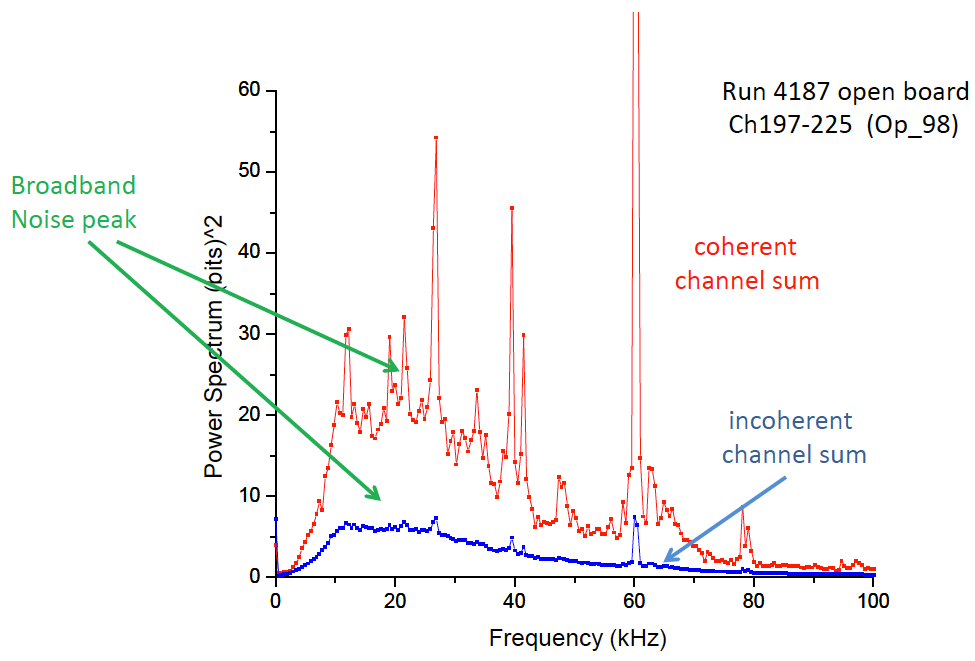
\includegraphics[keepaspectratio=true,width=\textwidth]{APDNoisePowerSpectrum.png}
\end{center}
\renewcommand{\baselinestretch}{1}
\small\normalsize
\begin{quote}
\caption{Coherent and incoherent noise power spectra for a sample set of APD channels without pulse shaping.  The coherent noise power spectrum is measured by adding together waveforms from different channels and computing a power spectrum; the incoherent noise power spectrum is measured by computing power spectra for each channel individually and adding them together~\cite{ElectronicsUpgradeReport}.}
\label{fig:APDNoisePowerSpectrum}
\end{quote}
\end{figure}
\renewcommand{\baselinestretch}{2}
\small\normalsize

The design goal of EXO-200 was for individual APD channels to have root-mean-square noise levels of 2000 electrons, and this goal was met~\cite{ElectronicsUpgradeReport}.  However, rather than observing the noise on summed APD channels increase proportionally to the square root of the number of channels, the summed APD noise is roughly two to three times higher than projected.  Figure~\ref{fig:APDNoisePowerSpectrum} compares the power spectrum of the summed APD waveforms to the sum of power spectra of individual APD waveforms; the power spectrum of the sum is 2-3 times higher than the sum of power spectra.  These observations indicate that the phases of the noise frequency components on different channels are positively correlated, leading to a worse impact on energy resolution than the same level of uncorrelated noise would give.

\begin{figure}
\begin{center}
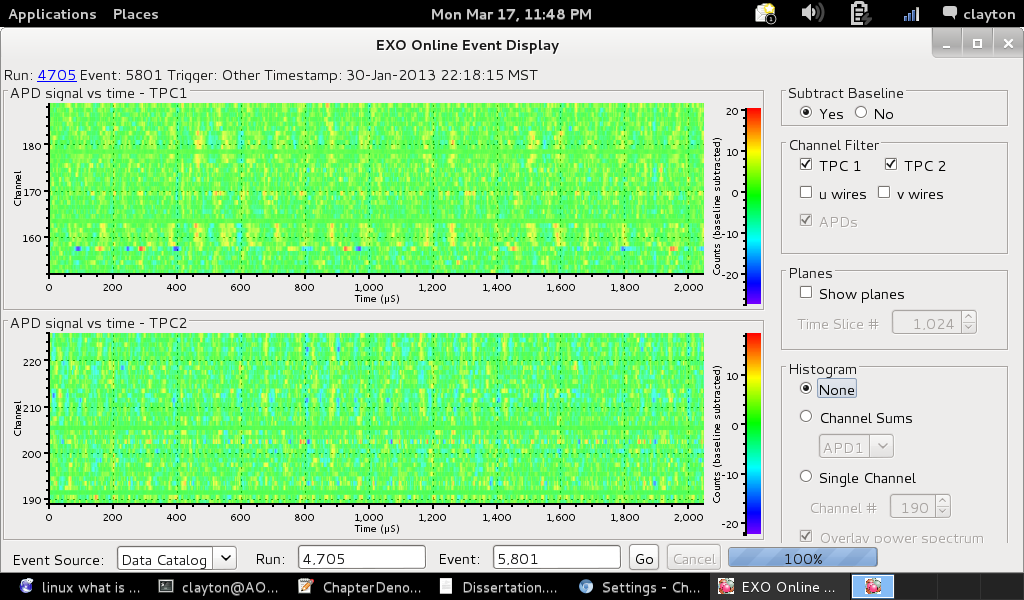
\includegraphics[keepaspectratio=true,width=\textwidth,clip=true,trim=1mm 21mm 91mm 24mm]{Run4705Ev5801_noiseEventDisplay.png}
\end{center}
\renewcommand{\baselinestretch}{1}
\small\normalsize
\begin{quote}
\caption{APD waveforms from a single event.  No energy deposit occured during this event, so the waveforms represent pure electronic noise.  The horizontal axis indicates time, and the vertical axis indicates channel number; colors ranging from blue to red indicate the baseline-subtracted waveform magnitude.  Vertical streaks are indicative of correlations in noise across channels.}
\label{fig:EvtDisplay_APDNoise}
\end{quote}
\end{figure}
\renewcommand{\baselinestretch}{2}
\small\normalsize

The correlations in noise across channels are visible even by eye.  Figure~\ref{fig:EvtDisplay_APDNoise} shows a single noise event from the detector taken on January 30, 2013, when noise levels were near their highest.  The horizontal axis represents time, the vertical axis represents channel number, and color indicates the magnitude of the baseline-subtracted waveform.  If noise on different channels were uncorrelated, we should see no relation between the noise on different horizontal rows (channels) of the plot.  Instead, vertical streaks can be seen which indicate noise which is in phase across multiple channels.

The observation that noise is correlated across channels has provided an important clue to the origin of the noise, and investigations led to the discovery that switching power supplies and a switched voltage regulator introduce noise into the electronics; these are magnified by a ground loop in the electronics and a pre-amplifier design which is not optimized to reject noise in its power supply.  Efforts are underway to address these issues in hardware~\cite{ElectronicsUpgradeReport_Dec2013,ElectronicsUpgradeReport_March2014}.

The observation that coherent APD electronic noise is the limiting factor in our energy resolution also implies that we can mitigate this noise in offline analysis.  Although the correlations in noise initially worsen our energy resolution due to their linear scaling with the number of channels, knowledge of these correlations will permit us to take advantage of the redundancy in the noise and reduce its overall magnitude.  By observing that the majority of our APD noise is correlated, we have learned that we can eliminate the majority of our APD noise in offline analysis and improve the quality of data which has already been taken.  Efforts to denoise the data in this way have been made by many members of the EXO collaboration; here we describe the success of one of these denoising approaches.

Although the previous discussion emphasizes the electronic noise which induces time variations in our energy resolution, we note that this is not the only source of noise in APD waveforms.  The types of noise which will be considered in the present work are:
\begin{itemize}
\item Electronic noise.  More generally, we consider collectively additive noise which is uncorrelated with pulses.  APD dark current is another possible source of such noise.
\item Fluctuations in photon collection efficiency.
\item Fluctuations in APD gain.
\end{itemize}
The last two will sometimes collectively be described as Poissonian noise because they each will introduce a variance term which is roughly linear in the energy of the event.

We note that the electronic noise will scale linearly with the number of channels used, in the case where it is dominated by coherent noise; by contrast, Poissonian noise will decrease proportionally to the square root of the number of channels used, in the case where all channels are expected to have similar mean photon collection and gain.  Thus, there are competing forces to form our energy estimates from a small number of channels to minimize the electronic noise and from a large number of channels to minimize the Poissonian noise.  Finding the optimal balance between these two extremes will be one of the challenges of denoising.

The energy estimator which we derive in this chapter is an optimal linear estimator, and we do not attempt to control how it produces its estimates.  However, we still can identify a number of qualitative approaches to reducing the noise levels in the scintillation channel.  We refer to ``passive" approaches as those in which components of our waveforms are weighted based on their relative signal-to-noise content.  ``Active" approaches, by contrast, are classified as those which attempt to improve the signal-to-noise content of the waveforms.  We identify the following three types of denoising:
\begin{description}
\item[Frequency weighting] \hfill \\
On a given channel waveform, weight more heavily the frequency components which contain larger signal-to-noise ratio.  This passive denoising scheme requires knowledge of the power spectra of the pulse signal and the noise.

\item[Channel weighting] \hfill \\
Different channels may have differing levels of noise, so some may generally have lower signal-to-noise ratios.  More importantly, though, the pulse magnitude on a given channel depends strongly on the proximity of the APD gang to the source of scintillation within the detector.  This passive denoising scheme therefore consists of weighting more heavily the channels which have larger expected pulse magnitudes, as determined on an event-by-event basis.

\item[Noise cancellation] \hfill \\
This active form of denoising consists of using correlations between noise on multiple channels to produce a better estimate of the noise component of waveforms than each waveform taken independently could provide.  To accomplish this, we require detailed information about the pairwise noise correlations across channels at each frequency.
\end{description}

Section~\ref{sec:DenoisingNotationSetup} specifies the mathematical framework for denoising.  This framework is general enough to include all of the features described in this section.

\section{Notational Conventions and External Input}\label{sec:DenoisingNotationSetup}

In this section, we first establish a set of notational conventions which will clarify the mathematics of this chapter.  We then describe the overarching framework in which denoising will take place, taking care that the framework is general enough to include all of the qualitative features described in section~\ref{sec:WhatIsDenoising}.

Throughout this chapter we use the following notational conventions:
\begin{itemize}
\item $i$, $j$ will represent indices over APD channels (or equivalently, APD gangs).
\item $a$, $b$, $c$ will represent indices of scintillation clusters in an event; a scintillation cluster is a set of simultaneous energy deposits which may occur at multiple locations.
\item $\tau$ will represent the time indices of a discrete-time waveform; $t_a$ represents the calendar time of a scintillation deposit $a$.
\item $f$, $g$ will represent the frequency indices of Fourier-transformed waveforms.
\item $\delta_{ij}$ is the Kronecker delta, equal to 1 if $i = j$ and 0 otherwise.
\item For a waveform $*[\tau]$, we will represent the discrete Fourier transform of that waveform with $\widetilde{*}[f]$, where the particular convention used to evaluate the Fourier transform is not significant.
\item For a Fourier-transformed waveform $\widetilde{*}[f]$, we denote the real and imaginary parts of that waveform by $\widetilde{*}^R[f]$ and $\widetilde{*}^I[f]$, respectively.
\item For an unknown parameter $p$, the symbol $\widehat{p}$ will identify an estimator for $p$.
\item For an expression $f(\cdot)$ containing random variables, $\left<f(\cdot)\right>$ is the expectation value of $f(\cdot)$.  Here the expectation value will be meant in a frequentist sense: if we could repeat the experiment of generating the same number of initial photons in the same places, $\left<f(\cdot)\right>$ would be the average value of $f(\cdot)$ from many trials of this hypothetical experiment.  The expectation value of $f(\cdot)$ conditional on the value of some random variable X is written $\left<f(\cdot) \middle\vert X\right>$.
\item When a bare index appears on both sides of an equation, the equation holds for all possible values of that index; for example, $f_i(\cdot) = g_i(\cdot)$ would mean that for all possible indices $i$ the equation holds.
\item Einstein notation is not used; all summations are written explicitly.
\item All energies will be in units of 2615 keV (the energy of the $^{208}$Tl gamma line).  This energy scale is natural for us because the lightmap of chapter~\ref{ch:Lightmap} is measured with events from that gamma line.
\end{itemize}

We describe the data as a collection of discretely sampled waveforms, $X_i[\tau]$.  We assume that all pulse times and shapes are already known, and only their magnitudes need to be extracted; so we can model the waveforms by
\begin{equation}\label{eqn:TimeDomainModelEquation}
X_i[\tau] = \sum_a M_{ia}Y_{ia}[\tau] + N_i[\tau] + b_i,
\end{equation}
where $Y_{ia}[\tau]$ is the template function of the pulse caused by scintillation cluster $a$ on channel $i$, $M_{ia}$ is the unknown magnitude of that pulse, and $N_i[\tau]$ and $b_i$ represent the electronic noise and baseline, respectively, of the channel.

\begin{figure}
\begin{center}
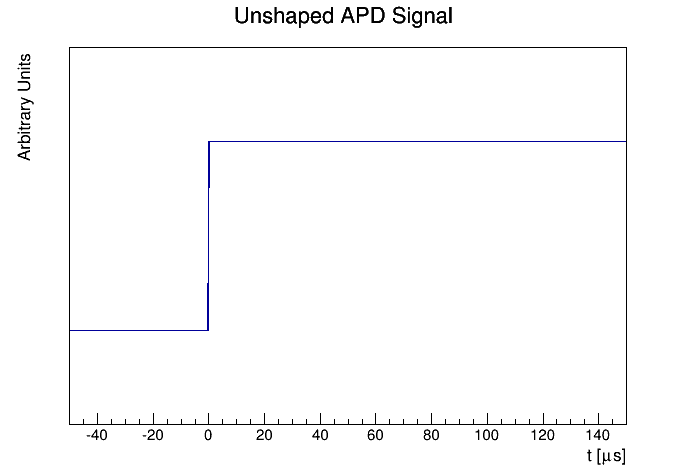
\includegraphics[keepaspectratio=true,width=4in]{scripts/UnshapedAPDWaveform.png}
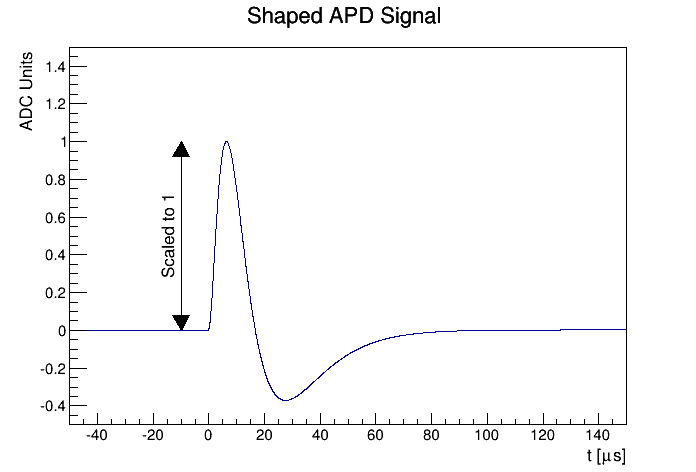
\includegraphics[keepaspectratio=true,width=4in]{scripts/ShapedAPDWaveform.png}
\end{center}
\renewcommand{\baselinestretch}{1}
\small\normalsize
\begin{quote}
\caption{Shaped and unshaped APD waveforms.  The normalization is shown to make the peak of the shaped waveform have a magnitude of one, and the time axis is shifted so that the unshaped waveform is a step function centered at $t=0$.}
\label{fig:SampleAPDTemplates}
\end{quote}
\end{figure}
\renewcommand{\baselinestretch}{2}
\small\normalsize

To break the degeneracy between $M$ and $Y$ we must fix the magnitude of the template function $Y$.  We choose to require that the function $Y$ has a baseline of zero and a peak magnitude of one, as illustrated in figure~\ref{fig:SampleAPDTemplates}.

The magnitude of a pulse is a random variable which depends on both the energy of the scintillation cluster and on random fluctuations detailed in section~\ref{sec:DescriptionOfPhotonNoise}.  We assume that the expected magnitude $\left<M_{ia}\right>$ of a pulse on channel $i$ from a single-site $2615$-keV deposit is known, and is characterized as a function $L_i(\vec{x}_a, t_a)$ of the deposit position $\vec{x}_a$ and calendar time $t_a$.  We can thereby characterize the expected yields $M_{ia}$ from a scintillation cluster with energy $E_a$ (in units of 2615 keV) as:
\begin{equation}\label{eqn:DefineLByEandM}
\left< M_{ia} \right> = L_i(\vec{x}_a, t_a) E_a.
\end{equation}
The exact methods for measuring $L_i(\vec{x}, t)$ will be described in chapter~\ref{ch:Lightmap}.

In cases where a multi-site scintillation cluster deposits energy in multiple locations, we use the charge information to estimate the energy deposited in each location; the estimated lightmap yield $L_i^{MS}$ from a multi-site scintillation cluster will be a weighted sum:
\begin{equation}
L_i^{MS}(\vec{x}_1, \dots, \vec{x}_{n_{max}}, t) = \frac{\sum_n E_n^{charge} L_i(\vec{x}_n, t)}{\sum_n E_n^{charge}},
\end{equation}
where the index $n$ ranges over the charge clusters associated with this scintillation cluster.  For notational simplicity, we will still write the expected yield on a channel $i$ from a multi-site scintillation cluster as $L_i(\vec{x}, t)$; in practice it will always be clear how to compute the expected yields for any scintillation cluster from this function.

For describing the electronic noise, it is much simpler to characterize its properties in frequency space, so we take the Fourier transform of equation~\ref{eqn:TimeDomainModelEquation} and drop the zero-frequency component (which only serves as a measure of the baseline $b_i$) to obtain
\begin{equation}\label{FrequencyDomainModelEquation}
\widetilde{X}_i[f] = \sum_a M_{ia}\widetilde{Y}_{ia}[f] + \widetilde{N}_i[f].
\end{equation}
We characterize the electronic noise by its second moments.  It will be computationally useful to decompose complex-valued numbers into their rectangular coordinates, so our characterization of the electronic noise should include the expectation values of:
\begin{subequations}\label{eq:FirstStatementOfNoiseCorrelations}\begin{align}
&\left< \widetilde{N}^R_i[f]\widetilde{N}^R_j[f] \right> \\
&\left< \widetilde{N}^R_i[f]\widetilde{N}^I_j[f] \right> \\
&\left< \widetilde{N}^I_i[f]\widetilde{N}^R_j[f] \right> \\
&\left< \widetilde{N}^I_i[f]\widetilde{N}^I_j[f] \right>,
\end{align}\end{subequations}
for all pairs $i$, $j$ of APD channels and all non-zero frequency components $f$.  Correlations between noise in different frequencies, $\left<\widetilde{N}_i[f]\widetilde{N}_j[g]\right>$ where $f \ne g$, are always equal to zero.  The measurement of these correlations will be described in chapter~\ref{ch:NoiseMeasurements}; this chapter will simply presume that they are known.

\section{APD Noise Model: the Photon Perspective}\label{sec:DescriptionOfPhotonNoise}

In this section we describe a model for the Poissonian noise which comes from fluctuations in photon collection and APD gain.  The model is constructed from a physical understanding of the APDs, and includes a step-by-step breakdown of where noise is introduced at each stage of the light collection process.  For reference, the reader is referred to section~\ref{sec:DetectorReadout} which describes the readout process, including the operation of APDs.

We define $P_a^{(0)}$ to be the initial number of photons generated by scintillation cluster $a$; this parameter is an unknown non-random parameter.  Subsequent steps in the readout process will result in $P_{ia}^{(n)}$ quanta (photons, electron-hole pairs, or electrons) on channel $i$, where $n$ indicates the step of the readout process; this quantity is a function of $P_a^{(0)}$ and also incorporate the randomness of photon collection and gain fluctuations, so $P_{ia}^{(n)}$ is a random parameter whose distribution reflects the unknown non-random parameter $P_a^{(0)}$.  We now describe the readout stages.

First, each APD gang $i$ has some number $P^{(1)}_{ia}$ of photons which reach its active surface.  The mean fraction of photons reaching a particular gang $i$ from position $\vec{x}_a$ is written $f_i(\vec{x}_a)$ and is assumed to be known; however, the initial paths of the optical photons emitted from the source, their trajectories through the xenon, and their success in reflecting off of teflon surfaces are all random, so $P^{(1)}_{ia}$ is a Poisson-distributed random variable with mean $f_i(\vec{x}_a)P^{(0)}_a$.  A typical $\beta\beta 0\nu$ event may deposit up to $\sim 1000$ photons on a nearby APD gang, resulting in roughly $3\%$ uncertainty from photon statistics; for a deposit in the bulk of the xenon, individual APD gangs may collect only one-tenth of this number of photons, resulting in closer to $10\%$ uncertainty due to photon statistics on the nearest APD gang.  Thus, we find that the noise on a single APD channel due to photon collection fluctuations may be quite significant.

Additionally, the numbers of photons reaching different gangs are not uncorrelated; since a photon which reaches gang $i$ cannot deposit on a different gang $j$, $P^{(1)}_{ia}$ and $P^{(1)}_{ja}$ are anticorrelated for different gangs $i \ne j$.  This process is described by a multinomial distribution.  Explicitly, the expectation values of our multinomial distribution are known to be:~\cite{ProbabilityTextbook}
\begin{IEEEeqnarray}{cCl}\label{eqn:CorrelationsOfP1}
\left< P^{(1)}_{ia} \right> &=& f_i(\vec{x}_a)P^{(0)}_a \IEEEyesnumber\IEEEyessubnumber\label{eqn:MeanOfP1}\\
\left< P^{(1)}_{ia} P^{(1)}_{jb} \right> &=& \left< P^{(1)}_{ia} \right> \left< P^{(1)}_{jb} \right> + \left[ f_i(\vec{x}_a)\delta_{ij} - f_i(\vec{x}_a)f_j(\vec{x}_a) \right] P^{(0)}_a \delta_{ab} \IEEEyessubnumber
\end{IEEEeqnarray}

(As a detail, we should note that the multinomial distribution is an incorrect model in one important respect: a photon may reflect off of teflon one or more times on its way to the APD.  Photons incident on the teflon may be absorbed, which would lead to a reflection efficiency which is less than one.  Furthermore, it is possible that teflon is be mildly fluorescent at the wavelength of our scintillation, leading to an increase in reflection efficiency.  Combining the variances which come from each segment on a photon's trajectory and the variances from fluctuations in the reflection efficiency of teflon can be done with the conditional variance formula~\cite{ProbabilityTextbook}, but we currently have no estimate of the number of reflections a photon will undergo.  The consequence is that we probably mis-estimate the variance of $P^{(1)}_{ia}$.)

Next, photons which arrive at the active surface of an APD must convert to electron-hole pairs in the silicon semiconductor layer of the APD; see section~\ref{sec:DetectorReadout} for details.  The energy required to produce one electron-hole pair in silicon is $3.66$ eV, so each incident photon produces roughly $1.9$ electron-hole pairs. We will define $P^{(2)}_{ia}$ to be the number of electron-hole pairs actually produced from $P^{(1)}_{ia}$ incident photons.  The Fano factor for electrons produced in silicon is roughly $0.1$, meaning that in addition to the uncertainty in $P^{(1)}_{ia}$ which we have already characterized, there is an additional uncorrelated variance in $P^{(2)}_{ia}$ equal to $0.1 \left<P^{(2)}_{ia}\right>$~\cite{EXOLAAPD}.  The correlations in the parameters $P^{(2)}_{ia}$ are therefore:
\begin{IEEEeqnarray}{cCl}\label{eqn:CorrelationsOfP2}
\left< P^{(2)}_{ia} \middle\vert P^{(1)}_{ia}\right> &=& 1.9 \cdot P^{(1)}_{ia} \IEEEyesnumber\IEEEyessubnumber \label{eqn:MeanOfP2}\\
\left< P^{(2)}_{ia} P^{(2)}_{jb} \middle\vert P^{(1)}_{ia}, P^{(1)}_{jb} \right> &=& (1.9)^2\cdot P^{(1)}_{ia} P^{(1)}_{jb}  + 0.1 \cdot 1.9 \cdot P^{(1)}_{ia} \delta_{ij}\delta_{ab} \IEEEyessubnumber \label{eqn:VarOfP2}
\end{IEEEeqnarray}

Electron-hole pairs are then amplified by an avalanche process inside the APDs.  The magnitude of this gain is APD-dependent, generally on the order of $200-300$, and can be identified by a time-dependent quantity $G^D_i(t)$ (where $D$ stands for diode); we will call the number of output electrons $P^{(3)}_{ia}$.  In addition to amplification of existing noise in $P^{(2)}_{ia}$, two additional source of noise are introduced:
\begin{itemize}
\item First, there is statistical variance in the amplification experienced by each electron due to the randomness of the avalanche process.  This variance is dependent on many factors, including the gain, and scales linearly with the number of electrons; we define the variance on the gain experienced by a single electron on channel $i$ as $\sigma^2_{G_i}(t)$.  From~\cite{EXOLAAPD}, $\sigma^2_{G_i}(t)$ is approximately equal to $\left(G^D_i(t)\right)^2$ when $G^D_i(t)=100$; as a result, we approximate
\begin{equation}\label{eqn:GainFluctuationEstimate}
\sigma^2_{G_i}(t) \approx \left(G^D_i(t)\right)^2.
\end{equation}
\item Second, there are gain non-uniformities in the diode volume, which contribute variance proportional to the square of the number of initial electron-hole pairs; we will identify the proportionality constant as $\sigma^2_{NU}$, which may depend on time and APD gang.  The magnitude of this uncertainty is not well-known, but may be significant.  In particular, the ganging together of APDs means that a single channel is a sum of pulses which have been exposed to six or seven different gain factors from the different APDs in that gang; the diameter of an APD gang is 58 mm~\cite{detectorPartI}, and gain non-uniformity is expected to be a significant factor when photons deposit preferentially on one portion of that area.  Our current code base treats $\sigma^2_{NU}$ as zero; however, future analyses will likely attempt to estimate it, and the derivation which follows retains it as an aid to that anticipated work.
\end{itemize}
These fluctuations are not correlated across channels, so their variances are multiplied by $\delta_{ij}\delta_{ab}$ to ensure they only contribute to variance terms and not covariance terms.  The correlations in the parameters $P^{(3)}_{ia}$ are therefore:
\begin{IEEEeqnarray}{cCl}\label{eqn:CorrelationsOfP3}
\left< P^{(3)}_{ia} \middle\vert P^{(2)}_{ia}\right> &=& G^D_i(t_a)P^{(2)}_{ia} \IEEEyesnumber\IEEEyessubnumber \label{eqn:MeanOfP3}\\
\left< P^{(3)}_{ia} P^{(3)}_{jb} \middle\vert P^{(2)}_{ia}, P^{(2)}_{jb}\right> &=& G^D_i(t_a)G^D_j(t_b) P^{(2)}_{ia} P^{(2)}_{jb} + \left[P^{(2)}_{ia}\sigma^2_{G_i}(t_a) + \left(P^{(2)}_{ia}\right)^2\sigma^2_{NU}\right]\delta_{ij}\delta_{ab} \nonumber \\* \IEEEyessubnumber\label{eqn:VarOfP3}
\end{IEEEeqnarray}

Finally, there is amplification $G^E_i(t)$ associated with the electronics of the APDs which is dependent on time and channel.This includes preamplifier gain, shaper gain, gain associated with the shaping times, and conversion from voltage to ADC counts.  We assume that this gain does not suffer any fluctuations, so no new variance is produced.  The output from this amplification is a waveform in ADC counts, so we can link it to the magnitude variable $M_{ia}$ of equation~\ref{FrequencyDomainModelEquation} by stating that:
\begin{IEEEeqnarray}{cCl}\label{eqn:DefnOfMFromP3}
\left<M_{ia} \middle\vert P^{(3)}_{ia}\right> &=& G^{E}_i(t_a) P^{(3)}_{ia} \IEEEyesnumber\IEEEyessubnumber\\
\left<M_{ia}M_{jb} \middle\vert P^{(3)}_{ia}, P^{(3)}_{jb}\right> &=& G^{E}_i(t_a)G^E_j(t_b) P^{(3)}_{ia} P^{(3)}_{jb}. \IEEEyessubnumber
\end{IEEEeqnarray}
Although we assume that no noise correlated with pulses is introduced during this stage, there is electronic noise $N_i[\tau]$ introduced at this stage which has been described above and is uncorrelated with the pulses.  Additionally, the APDs can contribute noise in the form of a dark current which is uncorrelated with pulses; this is inseparable from the electronic noise, and so we absorb it into our description of $N_i[\tau]$.

Equations~\ref{eqn:CorrelationsOfP1}, \ref{eqn:CorrelationsOfP2}, \ref{eqn:CorrelationsOfP3}, and \ref{eqn:DefnOfMFromP3} collectively chart the mean and variance of the APD pulse magnitudes at each step of readout and amplification.  We can eliminate the intermediate terms $P^{(1)}_{ia}$, $P^{(2)}_{ia}$, and $P^{(3)}_{ia}$ by substitution and obtain a full description for the first and second moments of the pulse magnitudes $M_{ia}$, $M_{jb}$ depending only on the unknown numbers of emitted photons $P^{(0)}_a$, $P^{(0)}_b$ and not on any random variables:
\begin{IEEEeqnarray}{cCl}\IEEEyesnumber\phantomsection\label{eqn:DefnOfMFromP0}
\left<M_{ia} \right> &=& 1.9 \cdot G_i(t_a) f_i(\vec{x}_a) P^{(0)}_a \IEEEyessubnumber\label{eqn:DefnOfMFromP0_Mean}\\
\left<M_{ia}M_{jb}\right> &=& (1.9)^2 \cdot G_i(t_a) G_j(t_b) f_i(\vec{x}_a)f_j(\vec{x}_b) P^{(0)}_a P^{(0)}_b\left(1 + \frac{\sigma_{NU}^2}{\left(G_i^D(t_a)\right)^2} \delta_{ij}\delta_{ab}\right) \nonumber \\
& & {}- (1.9)^2 \cdot G_i(t_a)G_j(t_a) f_i(\vec{x}_a)f_j(\vec{x}_a)P^{(0)}_a \delta_{ab} \IEEEyessubnumber\\
& & {}+ (1.9)\cdot G_i(t_a) G^E_i(t_a)f_i(\vec{x}_a) P^{(0)}_a \delta_{ij}\delta_{ab} \left[ (1.9 + 0.1)G_i^D(t_a) + \frac{\sigma^2_{G_i}(t_a)}{G_i^D(t_a)}\right],\nonumber
\end{IEEEeqnarray}
where for notational convenience we have defined $G_i(t) = G_i^E(t)G_i^D(t)$ as the product of the electronic and APD gains.

A simple substitution is possible by the property of conditional expectations, which states that the expectation value of a random value $X$ is the same as the result from taking an expectation value of $X$ conditional on $Y$ followed by an expectation value of the result:~\cite{ProbabilityTextbook}
\begin{equation}
\left<X \right> = \left< \left< X \middle\vert Y\right>\right>.
\end{equation}
The choice throughout to convey second moments of random variables with expectation values, as $\left<XY\right>$, rather than with covariances as $\mathrm{cov}(X,Y)$, is for the simplicity this provides; had we chosen to use covariances, combining these separate results would have required the use of the conditional covariance formula:~\cite{ProbabilityTextbook}
\begin{equation}
\mathrm{cov}(X,Y) = \left<\mathrm{cov}(X,Y \vert Z)\right> + \mathrm{cov}(\left<X\middle\vert Z\right>, \left<Y\middle\vert Z\right>.
\end{equation}
So, simplicity has been gained by avoiding a description of the model in terms of covariances.

Equations~\ref{eqn:DefnOfMFromP0} fully characterize the first and second moments of the random variables $M_{ia}$, which are the magnitudes of the observed pulses.  This is a key step in building a full model of the APD noise.  However, the expressions for these first and second moments are in terms of some parameters which are not directly observable.  In particular, we do not have the ability to directly measure the function $f_i(\vec{x})$ which describes the average fraction of photons which arrive on channel $i$ from an initial position $\vec{x}$.  In section~\ref{sec:BridgePhotonsPulses} we will restate equations~\ref{eqn:DefnOfMFromP0} in terms of quantities which are directly observable so that it is usable in practice.

\section{Bridge between Photons and Pulses}\label{sec:BridgePhotonsPulses}

We have characterized in equation~\ref{eqn:DefnOfMFromP0} the first and second moments of the random variables $M_{ia}$.  However, that characterization is phrased in terms of quantities which are not observable, so its practical utility is limited.  In this section we transform equation~\ref{eqn:DefnOfMFromP0} into a form which is usable in practice, and identify where we obtain the key parameters which it contains.

The main part of equation~\ref{eqn:DefnOfMFromP0} which we are unable to access experimentally is $f_i(\vec{x})$, the fraction of photons originating from position $\vec{x}$ which will arrive at APD channel $i$.  However, we do have observations of a related quantity: in equation~\ref{eqn:DefineLByEandM} we make use of a lightmap function $L_i(\vec{x}, t)$ which identifies the average magnitude (in ADC counts) of a pulse on channel $i$ produced from a 2615-keV energy deposit at position $\vec{x}$ and calendar time $t$ (where 2615 keV is selected because we measure it from the 2615-keV $^{208}$Tl gamma line of our thorium source calibrations).  Chapter~\ref{ch:Lightmap} describes how this lightmap function is measured from data; here we simply note that, because $L_i(\vec{x}, t)$ relates deposited energy to measured pulse sizes without reference to the number of photons internally created, it is possible to measure it directly from data.

Additionally, we must relate the quantity of energy deposited to the number of photons produced.  This is not directly measurable in the EXO-200 detector, so we must rely on simulation to estimate it; however, in section~\ref{sec:DerivationOfEstimator} we find that this relation will not have an impact on our energy estimator, so it need not be precise.  Simulations using NEST~\cite{NESTpaper} which have been performed within the EXO group by Liangjian Wen at our bulk electric field of 376 V/cm indicate that we can expect $82,000$ photons from a $2615$-keV gamma deposit.  We identify this ratio between photons generated and energy deposited with the parameter $c \approx 82,000$, and express the average relation between energy and photon yield in EXO-200 by
\begin{equation} \label{eqn:DefnOfP0}
P^{(0)}_a = c \cdot E_a,
\end{equation}
where $E_a$ is the energy of scintillation cluster $a$ in units of 2615 keV.

Equation~\ref{eqn:DefnOfP0} is treated here as exact, but this may not be so.  It is likely that photon yield does not scale linearly with energy; additionally, there are fluctuations in the number of photons produced for a particular energy deposit, and we are not treating $P^{(0)}_a$ as a random variable depending on $E$.  The essential point here is that the scintillation ``energy'' which we measure with the APD waveforms is a direct reflection of the number of photons $P^{(0)}_a$, and only indirectly reflects the true scintillation cluster energy $E_a$.  Similarly, the ionization energy measurement which is made with the u-wires is a direct reflection of the number of free electrons generated, and only indirectly reflects the true deposit energy.  The purpose of the energy calibration, described in section~\ref{sec:ResultEnergy}, is to combine our estimates of scintillation energy (proportional to the number of photons) and ionization energy (proportional to the number of free electrons) into a single estimate of the true deposited energy, taking into account any non-linearities in either component.  We find it convenient to report the scintillation energy as $P^{(0)}_a/c$ rather than the true number of photons $P^{(0)}_a$, so the reported scintillation energy is roughly comparable to the true amount of deposited energy; but our goal is still only to measure (a quantity proportional to) the number of photons created.  In the derivations of this chapter we will refer to $E_a$ as the energy of scintillation cluster $a$, but it is the scintillation energy, not the true deposited energy, which we mean by this variable.

We can now combine equations~\ref{eqn:DefineLByEandM}, \ref{eqn:DefnOfMFromP0_Mean}, and \ref{eqn:DefnOfP0} to relate $f_i(\vec{x})$ and $L_i(\vec{x}, t)$:
\begin{equation}\label{eqn:RelationLandF}
L_i(\vec{x}, t) = 1.9 \cdot c f_i(\vec{x}) G_i(t).
\end{equation}
We use this relation and equation~\ref{eqn:DefnOfP0} to eliminate $f_i(\vec{x})$ from equation~\ref{eqn:DefnOfMFromP0} and restate the moments of the pulse magnitudes $M_{ia}$ as:
\begin{IEEEeqnarray}{cCl}\phantomsection\label{eqn:DefnOfMFromE}
\left<M_{ia} \right> &=& L_i(\vec{x}_a, t_a) E_a \IEEEyesnumber\IEEEyessubnumber\label{eqn:DefnOfMFromE_Mean}\\
\left<M_{ia}M_{jb}\right> &=& L_i(\vec{x}_a, t_a) L_j(\vec{x}_b, t_b) E_a E_b\left(1 + \frac{\sigma_{NU}^2}{\left(G_i^D(t_a)\right)^2} \delta_{ij}\delta_{ab}\right) \nonumber \\
& & {}- L_i(\vec{x}_a, t_a) L_j(\vec{x}_a, t_a) E_a \delta_{ab}/c \IEEEyessubnumber\\
& & {}+ L_i(\vec{x}_a, t_a)E_a \delta_{ij}\delta_{ab} \left[ (1.9 + 0.1)G_i(t_a) + \frac{G^E_i(t_a)}{G_i^D(t_a)}\sigma^2_{G_i}(t_a)\right].\nonumber
\end{IEEEeqnarray}

We will see in equation~\ref{eqn:SeparableLightmap} that the lightmap $L_i(\vec{x},t)$ is treated as a separable function, $L_i(\vec{x},t) = R_i(\vec{x})S_i(t)$.  The right hand side of equation~\ref{eqn:RelationLandF} has factors which depend strictly on either position or time, but not both; so we can separate the position-dependent and time-dependent factor from both sides and state:
\begin{subequations}\begin{align}
R_i(\vec{x}) &\propto f_i(\vec{x}) \\
S_i(t) &\propto G_i(t).\label{eqn:SProportionalToGProduct}
\end{align}\end{subequations}
So, we can use the lightmap to understand the time-dependent behavior of the product of electronic and APD gain, $G_i(t)$, for each channel; but we cannot use it to set the absolute scale, nor can we use it to understand separately $G_i^E(t)$ and $G_i^D(t)$.

Measurements of $G^E_i(t)$ are possible from internal charge injection runs, as described in section~\ref{sec:DetectorCalibration}.  However, using these runs in a uniform way is difficult.  Internal charge injection runs are only useful for understanding relative changes in the electronic gain over time, and an external charge injection run is needed to set an absolute scale for the gain.  The only APD external charge injection runs were taken in February 2011, and have not been analyzed since that time; also, since that time some APD electronics boards have been replaced, resetting the scale of the internal charge injection runs.  For the present analysis, the charge injection runs are not used to fix $G^E_i(t)$.

However, we can still derive an estimate for the electronic gain which is sufficient for the present analysis.  The electronic gain comes entirely from known electronic components; based on these electronic components, the preamplifier has a gain of 1/(5 pF), shapers have a combined 21.2, and the digitizer digitizes 12 bits (4096 ADC counts) for a 2.5 volt pulse.  Combining these factors, we will use a time-independent estimate:
\begin{equation}\label{eqn:ApproxForGE}
G^E_i(t) = 1.1 \cdot 10^{-3}\:\text{ADC}/\text{e}^-.
\end{equation}
Future work should include a more careful study of the charge injection runs to improve this estimate, but we use this value to perform the present analysis.  A consequence of this choice is that all time-dependence of $S_i(t)$ must be absorbed into $G^D_i(t)$, so we can strengthen equation~\ref{eqn:SProportionalToGProduct} to:
\begin{equation}\label{eqn:S_propto_GD}
S_i(t) \propto G_i^D(t).
\end{equation}

We also have independent measurements of the APD gains $G^D_i(t)$ available from laser calibration runs.  These special runs allow a laser to shine into the detector from a fixed point and with a stable amplitude while the bias voltages on the APDs are varied from an effective unity gain to our standard voltage settings.  Using these measurements, we are able to measure $G^D_i(t)$ at weekly intervals from September 2012 to the present time.  Before September 2012, some less-reliable laser data is available, but results from that data are not readily available as of this writing.

It would be possible, and should be a goal for future improvements, to make use of this full range of laser data.  However, the laser data provides a less uniform history of APD gains over the full data-taking window of EXO-200 from September 2011 to November 2013, and it is much easier to track time-dependent behavior from thorium source data which have been collected regularly throughout that period.  As a result, a compromise is used to characterize $G^D_i(t)$.  One particular laser run, run 4540 (taken on December 13, 2012), is used to fix $G^D_i(t_{4540})$, and equation~\ref{eqn:S_propto_GD} is used to extrapolated using thorium source data:
\begin{equation}\label{eqn:ApproxForGD}
G^D_i(t) \approx G^D_i(t_{4540}) \cdot S_i(t)/S_i(t_{4540}).
\end{equation}
This assumption makes use of the approximation that $G^E_i(t)$ is roughly constant in time, which is probably only accurate to one significant figure; therefore when an electronics change is made to a channel, we can expect that the accuracy of $G^D_i(t)$ is no better than one significant figure.  These results mean that we can also estimate with the same level of accuracy:
\begin{equation}
f_i(\vec{x}) \approx \frac{S_i(t_{4540})}{G^D_i(t_{4540})} \cdot \frac{R_i(\vec{x})}{1.9 \cdot c G^E_i(t)}.
\end{equation}

The set of inputs needed to use equations~\ref{eqn:DefnOfMFromE} are $L_i(\vec{x},t)$, $G_i^D(t)$, $G_i^E(t)$, $\sigma_{NU}^2$, $\sigma_{G_i}^2(t)$, and $c$.  The lightmap $L_i(\vec{x},t)$ is measured in chapter~\ref{ch:Lightmap}.  Our approximations for $G_i^D(t)$ and $G_i^E(t)$ have been described in equations~\ref{eqn:ApproxForGD} and \ref{eqn:ApproxForGE}, respectively.  $c \approx 82,000$ was identified for equation~\ref{eqn:DefnOfP0}.  We have stated that $\sigma_{NU}^2$ is set equal to zero for this analysis, and is retained in this work to facilitate future investigations.  Equation~\ref{eqn:GainFluctuationEstimate} has estimated $\sigma^2_{G_i}(t) \approx \left(G^D_i(t)\right)^2$.

Thus, we have specified fully the parameters needed as inputs to equations~\ref{eqn:DefnOfMFromE}.  We now have at our disposal a full model for the Poissonian noise on APD channels.  We are finally prepared with all tools necessary to derive an optimal energy estimator, and this is done in section~\ref{sec:DerivationOfEstimator}.

\section{Derivation of an Optimal Energy Estimator}\label{sec:DerivationOfEstimator}

It is now possible to specify the optimization criteria for generating an energy estimate from the APD waveforms.  We wish to identify an energy estimator which is unbiased and has a minimal expected error.  For the problem to remain tractable, we demand that the estimator be linear.  Furthermore, although the Fourier-transformed waveforms $\widetilde{X}_i[f]$ are complex-valued, we require that the energy estimate be strictly real-valued.  This section describes the optimization criteria and constraints for the energy estimator, and then proceeds to derive an optimal estimator satisfying those constraints.

We recall from equation~\ref{FrequencyDomainModelEquation} our model for the APD waveforms:
\begin{equation}\label{eqn:FrequencyDomainModelEquation2}
\widetilde{X}_i[f] = \sum_a M_{ia}\widetilde{Y}_{ia}[f] + \widetilde{N}_i[f],
\end{equation}
where $M_{ia}$ and $\widetilde{N}_i[f]$ are random variables with known probability distributions, we choose to drop the zero-frequency component, and the probability distribution of $M_{ia}$ reflects the energy parameter which we intend to estimate.  We therefore take the energy estimator $\widehat{E}_a$ for the energy of scintillation cluster $a$ to be of the form:
\begin{equation}
\widehat{E}_a = \sum_{if} A_{ia}[f] \widetilde{X}_i^R[f] + B_{ia}[f] \widetilde{X}_i^I[f],
\end{equation}
where we recall from section~\ref{sec:DenoisingNotationSetup} that $*^R$ and $*^I$ are the real and imaginary parts, respectively, of a complex-valued parameter.  This expression is one form for the most general real-valued linear functional on $X_i[f]$.  The goal of denoising is therefore reduced to identifying the optimal parameters $A_{ia}[f]$ and $B_{ia}[f]$ for this estimator.

The mean squared error $\epsilon^2_a$ in the energy estimate $\widehat{E}_a$ of $E_a$ is defined by:
\begin{equation}
\epsilon^2_a = \left< \left(\widehat{E}_a - E_a\right)^2\right>.
\end{equation}
Our goal is to minimize $\epsilon^2_a$ under the constraint of no bias, ie. that:
\begin{equation}\label{eqn:ConstraintForm1}
\left<\widehat{E}_a - E_a\right> = 0
\end{equation}
or, by substitution of equation~\ref{eqn:FrequencyDomainModelEquation2} and applying our knowledge of the expectation value of $M_{ia}$ from equation~\ref{eqn:DefnOfMFromE_Mean} and our knowledge that the noise terms have mean zero, the no-bias constraint is equivalent to:
\begin{equation}
\sum_{ifb}\left[A_{ia}[f] \widetilde{Y}_{ib}^R[f] + B_{ia}[f] \widetilde{Y}_{ib}^I[f]\right] L_i(\vec{x}_b,t_b) E_b = E_a.
\end{equation}
However, we will find that it is necessary to specify a slightly stronger constraint.  In particular, it is desirable to ensure that the constraints are as independent of energy as possible to reduce the need to input an estimated energy into our energy estimator; therefore we freely employ the stronger constraint
\begin{equation}
\sum_{if}\left[A_{ia}[f] \widetilde{Y}_{ib}^R[f] + B_{ia}[f] \widetilde{Y}_{ib}^I[f]\right] L_i(\vec{x}_b,t_b) = \delta_{ab} \text{~for all b,} \label{eqn:ConstraintForm3}
\end{equation}
which implies the earlier forms and leads to advantageous cancellations of terms.  Conceptually, this constraint is equivalent to saying that estimates of the energy $E_a$ of a scintillation cluster $a$ should be unbiased and independent of any other energies $E_b$ which are present on the same waveform.

We now proceed with the optimization.  We start by expanding $\epsilon^2_a$:
\begin{align}
\epsilon^2_a &= \left< \left(\widehat{E}_a - E_a\right)^2\right> \\
%
&= \left< \widehat{E}^2_a \right> - E_a \left<\widehat{E}_a\right> - \left< \widehat{E}_a - E_a \right> E_a \\
%
\intertext{We employ the constraint of equation~\ref{eqn:ConstraintForm1} to simplify the second term of this expansion, and eliminate the third altogether; we then proceed:}
%
\epsilon^2_a &= \left< \widehat{E}^2_a \right> - E^2_a \\
%
&= \left< \left(\sum_{if}\left[ A_{ia}[f] \widetilde{X}_i^R[f] + B_{ia}[f] \widetilde{X}_i^I[f]\right]\right)^2\right> - E^2_a \\
%
& \begin{aligned}= \bigg< \bigg(&
  \sum_{if} \left[ A_{ia}[f] \widetilde{N}_i^R[f] + B_{ia}[f] \widetilde{N}_i^I[f]\right] \\
  & + \sum_{ifb} \left[ A_{ia}[f] \widetilde{Y}_{ib}^R[f] + B_{ia}[f] \widetilde{Y}_{ib}^I[f]\right]M_{ib}  \bigg)^2 \bigg> - E^2_a
\end{aligned} \\
%
\intertext{The noise $\widetilde{N}$ and signal $M_{ia}$ are uncorrelated, so multiplicative cross-terms have an expectation value of zero:}
%
\epsilon^2_a &= \left< \left(\sum_{if} \left[ A_{ia}[f] \widetilde{N}_i^R[f] + B_{ia}[f] \widetilde{N}_i^I[f]\right]\right)^2\right> \nonumber \\
&\quad + \left<\left(\sum_{ifb} \left[ A_{ia}[f] \widetilde{Y}_{ib}^R[f] + B_{ia}[f] \widetilde{Y}_{ib}^I[f]\right]M_{ib} \right)^2 \right> - E^2_a \\
%
\intertext{Additionally, electronic noise cross-terms between different frequencies evaluate to zero:}
%
\epsilon^2_a &= \left< \sum_{ijf} \left[ A_{ia}[f] \widetilde{N}_i^R[f] + B_{ia}[f] \widetilde{N}_i^I[f]\right] \left[ A_{ja}[f] \widetilde{N}_j^R[f] + B_{ja}[f] \widetilde{N}_j^I[f]\right] \right> \nonumber \\
&\quad + \left<\left(\sum_{ifb} \left[ A_{ia}[f] \widetilde{Y}_{ib}^R[f] + B_{ia}[f] \widetilde{Y}_{ib}^I[f]\right]M_{ib} \right)^2 \right> - E^2_a \\
%
& \begin{aligned}
  = \sum_{ijf} \bigg[ & A_{ia}[f]A_{ja}[f] \left<\widetilde{N}_i^R[f]\widetilde{N}_j^R[f]\right> + A_{ia}[f]B_{ja}[f] \left<\widetilde{N}_i^R[f]\widetilde{N}_j^I[f]\right> \nonumber \\
  & + B_{ia}[f]A_{ja}[f] \left<\widetilde{N}_i^I[f]\widetilde{N}_j^R[f]\right> + B_{ia}[f]B_{ja}[f] \left<\widetilde{N}_i^I[f]\widetilde{N}_j^I[f]\right>\bigg] \end{aligned} \nonumber \\
&\quad + \sum_{\substack{ifb\\jgc}} \left[A_{ia}[f] \widetilde{Y}_{ib}^R[f] + B_{ia}[f] \widetilde{Y}_{ib}^I[f]\right]\left[A_{ja}[g] \widetilde{Y}_{jc}^R[g] + B_{ja}[g] \widetilde{Y}_{jc}^I[g]\right] \left<M_{ib}M_{jc}\right> - E^2_a \\
%
\intertext{We now expand $\left<M_{ib}M_{jc}\right>$ using equation~\ref{eqn:DefnOfMFromE} and take advantage of the stronger form of our constraint~\ref{eqn:ConstraintForm3} to simplify the expression:}
%
\epsilon^2_a & \begin{aligned}[t]
  = \sum_{ijf} \bigg[ & A_{ia}[f]A_{ja}[f] \left<\widetilde{N}_i^R[f]\widetilde{N}_j^R[f]\right> + A_{ia}[f]B_{ja}[f] \left<\widetilde{N}_i^R[f]\widetilde{N}_j^I[f]\right> \\
  & + B_{ia}[f]A_{ja}[f] \left<\widetilde{N}_i^I[f]\widetilde{N}_j^R[f]\right> + B_{ia}[f]B_{ja}[f] \left<\widetilde{N}_i^I[f]\widetilde{N}_j^I[f]\right>\bigg] \end{aligned} \nonumber \\
&\quad + \left( \sum_{ifb} \left[A_{ia}[f] \widetilde{Y}_{ib}^R[f] + B_{ia}[f] \widetilde{Y}_{ib}^I[f]\right] L_i(\vec{x}_b,t_b) E_b \right)^2 - E^2_a \nonumber \\
&\quad - \sum_b \left( \sum_{if} \left[A_{ia}[f] \widetilde{Y}_{ib}^R[f] + B_{ia}[f] \widetilde{Y}_{ib}^I[f]\right] L_i(\vec{x}_b,t_b) \right)^2 \frac{E_b}{c} \nonumber \\
&\quad \begin{aligned}
  + \sum_{ifgb} &\left[A_{ia}[f] \widetilde{Y}_{ib}^R[f] + B_{ia}[f] \widetilde{Y}_{ib}^I[f]\right]\left[A_{ia}[g] \widetilde{Y}_{ib}^R[g] + B_{ia}[g] \widetilde{Y}_{ib}^I[g]\right] \cdot \\
  & \begin{aligned}
    L_i(\vec{x}_b,t_b) E_b \bigg[ &(0.1 + 1.9) G^E_i(t_b) G^D_i(t_b) \\
    & + \frac{G^E_i(t_b)}{G^D_i(t_b)} \sigma^2_{G_i}(t_b) + L_i(\vec{x}_b,t_b) E_b \frac{\sigma^2_{NU}}{\left(G^D_i(t_b)\right)^2} \bigg]
\end{aligned} \end{aligned} \\
%
& \begin{aligned}
  = \sum_{ijf} \bigg[ & A_{ia}[f]A_{ja}[f] \left<\widetilde{N}_i^R[f]\widetilde{N}_j^R[f]\right> + A_{ia}[f]B_{ja}[f] \left<\widetilde{N}_i^R[f]\widetilde{N}_j^I[f]\right> \\
  & + B_{ia}[f]A_{ja}[f] \left<\widetilde{N}_i^I[f]\widetilde{N}_j^R[f]\right> + B_{ia}[f]B_{ja}[f] \left<\widetilde{N}_i^I[f]\widetilde{N}_j^I[f]\right>\bigg] \end{aligned} \nonumber \\
&\quad \begin{aligned}
  + \sum_{ib} &\left( \sum_f \left[A_{ia}[f] \widetilde{Y}_{ib}^R[f] + B_{ia}[f] \widetilde{Y}_{ib}^I[f]\right]\right)^2 \cdot \\
  & \begin{aligned}
    L_i(\vec{x}_b,t_b) E_b \bigg[ &(0.1 + 1.9) G^E_i(t_b) G^D_i(t_b) \\
    & + \frac{G^E_i(t_b)}{G^D_i(t_b)} \sigma^2_{G_i}(t_b) + L_i(\vec{x}_b,t_b) E_b \frac{\sigma^2_{NU}}{\left(G^D_i(t_b)\right)^2} \bigg]
\end{aligned} \end{aligned} \nonumber \\
&\quad - \frac{E_a}{c}
\end{align}

We are now in a position to evaluate the partial derivatives of $\epsilon^2_a$ with respect to the parameters $A_{ia}[f]$ and $B_{ia}[f]$.  They are:
\begin{subequations}\begin{align}
\frac{\partial \epsilon^2_a}{\partial A_{ia}[f]} &= 2 \sum_j \left[ A_{ja}[f] \left<\widetilde{N}_i^R[f]\widetilde{N}_j^R[f]\right> + B_{ja}[f] \left<\widetilde{N}_i^R[f]\widetilde{N}_j^I[f]\right>\right] \nonumber \\
&\quad \begin{aligned}
  + 2 \sum_{gb} & E_b\widetilde{Y}_{ib}^R[f] L_i(\vec{x}_b,t_b)\left[A_{ia}[g] \widetilde{Y}_{ib}^R[g] + B_{ia}[g] \widetilde{Y}_{ib}^I[g]\right] \cdot \\
  & \begin{aligned}
    \bigg[ &(0.1 + 1.9) G^E_i(t_b) G^D_i(t_b) \\
  & + \frac{G^E_i(t_b)}{G^D_i(t_b)} \sigma^2_{G_i}(t_b) + L_i(\vec{x}_b,t_b) E_b \frac{\sigma^2_{NU}}{\left(G^D_i(t_b)\right)^2} \bigg]
\end{aligned} \end{aligned}\\
%
\frac{\partial \epsilon^2_a}{\partial B_{ia}[f]} &= 2 \sum_j \left[ A_{ja}[f] \left<\widetilde{N}_i^I[f]\widetilde{N}_j^R[f]\right> + B_{ja}[f] \left<\widetilde{N}_i^I[f]\widetilde{N}_j^I[f]\right>\right] \nonumber \\
&\quad \begin{aligned}
  + 2 \sum_{gb} & E_b\widetilde{Y}_{ib}^I[f] L_i(\vec{x}_b,t_b)\left[A_{ia}[g] \widetilde{Y}_{ib}^R[g] + B_{ia}[g] \widetilde{Y}_{ib}^I[g]\right] \cdot \\
  & \begin{aligned}
    \bigg[ &(0.1 + 1.9) G^E_i(t_b) G^D_i(t_b) \\
  & + \frac{G^E_i(t_b)}{G^D_i(t_b)} \sigma^2_{G_i}(t_b) + L_i(\vec{x}_b,t_b) E_b \frac{\sigma^2_{NU}}{\left(G^D_i(t_b)\right)^2} \bigg]
\end{aligned} \end{aligned}
\end{align}\end{subequations}

We use Lagrange's method to minimize $\epsilon^2_a$ while satisfying our constraints; we define
\begin{equation}
C_{ab} = \sum_{if}\left[A_{ia}[f] \widetilde{Y}_{ib}^R[f] + B_{ia}[f] \widetilde{Y}_{ib}^I[f]\right] L_i(\vec{x}_b,t_b),
\end{equation}
where the indices of $C_{ab}$ are ordered, and restate the constraints of equation~\ref{eqn:ConstraintForm3} as
\begin{equation}
C_{ab} = \delta_{ab}.
\end{equation}
Then, the partial derivatives of these constrained expressions are:
\begin{subequations}\begin{align}
\frac{\partial C_{bc}}{\partial A_{ia}[f]} &= \widetilde{Y}^R_{ic}[f] L_i(\vec{x}_c,t_c) \delta_{ab} \\
\frac{\partial C_{bc}}{\partial B_{ia}[f]} &= \widetilde{Y}^I_{ic}[f] L_i(\vec{x}_c,t_c) \delta_{ab}
\end{align}\end{subequations}

Denoting the set of Lagrange multipliers for $\epsilon^2_a$ with $\lambda_{ab}$, where the indices are ordered, and allowing these parameters to absorb constant factors, we can at last identify the full set of linear equations describing the optimal energy estimator $\widehat{E}_a$:
\begin{subequations}\begin{align}
&\sum_j \left[ A_{ja}[f] \left<\widetilde{N}_i^R[f]\widetilde{N}_j^R[f]\right> + B_{ja}[f] \left<\widetilde{N}_i^R[f]\widetilde{N}_j^I[f]\right>\right]\nonumber\\
&+ \sum_{gb} \begin{aligned}[t]
  & E_b\widetilde{Y}_{ib}^R[f] L_i(\vec{x}_b,t_b)\left[A_{ia}[g] \widetilde{Y}_{ib}^R[g] + B_{ia}[g] \widetilde{Y}_{ib}^I[g]\right] \cdot \\
  & \left[ (0.1 + 1.9) G^E_i(t_b) G^D_i(t_b) + \frac{G^E_i(t_b)}{G^D_i(t_b)} \sigma^2_{G_i}(t_b) + L_i(\vec{x}_b,t_b) E_b \frac{\sigma^2_{NU}}{\left(G^D_i(t_b)\right)^2} \right] \end{aligned} \nonumber \\
&+ \sum_b \lambda_{ab} \widetilde{Y}^R_{ib}[f] L_i(\vec{x}_b,t_b) = 0 \qquad \qquad \qquad \qquad \quad \text{for each $i$, $f$}\\
%
&\sum_j \left[ A_{ja}[f] \left<\widetilde{N}_i^I[f]\widetilde{N}_j^R[f]\right> + B_{ja}[f] \left<\widetilde{N}_i^I[f]\widetilde{N}_j^I[f]\right>\right]\nonumber\\
&+ \sum_{gb} \begin{aligned}[t]
  & E_b\widetilde{Y}_{ib}^I[f] L_i(\vec{x}_b,t_b)\left[A_{ia}[g] \widetilde{Y}_{ib}^R[g] + B_{ia}[g] \widetilde{Y}_{ib}^I[g]\right] \cdot \\
  & \left[ (0.1 + 1.9) G^E_i(t_b) G^D_i(t_b) + \frac{G^E_i(t_b)}{G^D_i(t_b)} \sigma^2_{G_i}(t_b) + L_i(\vec{x}_b,t_b) E_b \frac{\sigma^2_{NU}}{\left(G^D_i(t_b)\right)^2} \right] \end{aligned} \nonumber\\
&+ \sum_b \lambda_{ab} \widetilde{Y}^I_{ib}[f] L_i(\vec{x}_b,t_b) = 0 \qquad \qquad \qquad \qquad \quad \text{for each $i$, $f$}\\
%
&\sum_{if}\left[A_{ia}[f] \widetilde{Y}_{ib}^R[f] + B_{ia}[f] \widetilde{Y}_{ib}^I[f]\right] L_i(\vec{x}_b,t_b) = \delta_{ab} \qquad \text{for each $b$}
\end{align}\end{subequations}

To simplify the notation, let us define a new function:
\begin{equation} \label{eqn:DefinitionOfQ}
q(i,b) := \begin{aligned}[t]
  \bigg( &(0.1 + 1.9) G^E_i(t_b) G^D_i(t_b) + \frac{G^E_i(t_b)}{G^D_i(t_b)} \sigma^2_{G_i}(t_b)\\
  &+ L_i(\vec{x}_b,t_b) E_b \frac{\sigma^2_{NU}}{\left(G^D_i(t_b)\right)^2}\bigg)L_i(\vec{x}_b, t_b) E_b
\end{aligned}
\end{equation}
which we note should be strictly positive if measured correctly (because all gains and lightmap values should be strictly positive, and all variances are non-negative).  Using this shorthand, we re-write our system of equations in the more compact form:
\begin{subequations} \label{eqn:SystemToSolve} \begin{align}
&\sum_j \left[ A_{ja}[f] \left<\widetilde{N}_i^R[f]\widetilde{N}_j^R[f]\right> + B_{ja}[f] \left<\widetilde{N}_i^R[f]\widetilde{N}_j^I[f]\right>\right] \notag \\
&+ \sum_{gb} \widetilde{Y}_{ib}^R[f] q(i,b) \left[A_{ia}[g] \widetilde{Y}_{ib}^R[g] + B_{ia}[g] \widetilde{Y}_{ib}^I[g]\right] \notag \\
&+ \sum_b \lambda_{ab} \widetilde{Y}^R_{ib}[f] L_i(\vec{x}_b,t_b) = 0 \qquad \qquad \qquad \qquad \quad \text{for each $i$, $f$}\\
%
&\sum_j \left[ A_{ja}[f] \left<\widetilde{N}_i^I[f]\widetilde{N}_j^R[f]\right> + B_{ja}[f] \left<\widetilde{N}_i^I[f]\widetilde{N}_j^I[f]\right>\right] \notag \\
&+ \sum_{gb} \widetilde{Y}_{ib}^I[f] q(i,b) \left[A_{ia}[g] \widetilde{Y}_{ib}^R[g] + B_{ia}[g] \widetilde{Y}_{ib}^I[g]\right] \notag \\
&+ \sum_b \lambda_{ab} \widetilde{Y}^I_{ib}[f] L_i(\vec{x}_b,t_b) = 0 \qquad \qquad \qquad \qquad \quad \text{for each $i$, $f$}\\
%
&\sum_{if}\left[A_{ia}[f] \widetilde{Y}_{ib}^R[f] + B_{ia}[f] \widetilde{Y}_{ib}^I[f]\right] L_i(\vec{x}_b,t_b) = \delta_{ab} \qquad \text{for each $b$}
\end{align} \end{subequations}

It is important to note here that energies $E_b$, which we are intending to measure, do in fact enter into this linear set of equations.  At first this would seem to demonstrate that the equations here are impossible to apply, but in fact they remind us that our Poissonian noise, which is correlated with the signal, is also dependent on the magnitude of that signal.  Statistical fluctuations in the number of photons observed on each APD, for instance, scale like the square root of the number of photons emitted.

We can see, then, that some estimate of energy is necessary to know the relative importance of different forms of noise.  But the constraint equation ensures that our estimate will be unbiased regardless of what energy estimates are fed into the system of equations, so we can be confident that it is only a rough estimate of the energy scale which is needed, and not worry that the optimization will be biased to estimate energies similar to the estimates we feed in.  For this purpose, it is sufficient to use the charge-only energy as an estimate of the scintillation-only energy.

The optimal energy estimator is now fully specified by the parameters $A_{ia}[f]$ and $B_{ia}[f]$ which solve equations~\ref{eqn:SystemToSolve}, and the theory of denoising is fully specified.  Sections~\ref{sec:MatrixFormulationOfDenoising}-\ref{sec:DenoisingComputationalConsiderations} will consider the computational aspects of solving for this energy estimator.

\section{Matrix Formulation of Denoising}\label{sec:MatrixFormulationOfDenoising}

Because the system of equations above is linear in $A_{ia}[f]$ and $B_{ia}[f]$, we wish to solve it as a matrix equation.  This requires, first, that we choose an ordering of the unknowns; the best ordering will be the one which groups nonzero entries into blocks, since this will allow us to make more efficient use of matrix libraries.  We define:
\begin{equation}
\vec{A}_a = (A_{1 1 a}, B_{1 1 a}, A_{2 1 a}, B_{2 1 a}, \dots, B_{i_{max} 1 a}, A_{1 2 a}, \dots, A_{1 f_{max} a}, A_{2 f_{max} a}, \dots, A_{i_{max} f_{max} a})
\end{equation}
so that the entries alternate between $A$ and $B$, iterating quickly through channels and more slowly through frequencies.  Note that only the $A$ terms are included for the maximum frequency; this is because $X_i[t]$ is real-valued, so $\widetilde{X}_i[0]$ and $\widetilde{X}_i[f_{max}]$ are real-valued as well.  We also will find it convenient to define the matrix:
\begin{equation}
\mathbf{A} = \begin{pmatrix}
\vdots & & \vdots \\
\vec{A}_1 & \cdots & \vec{A}_{a_{max}} \\
\vdots & & \vdots
\end{pmatrix}
\end{equation}
which includes the parameters needed for each of the estimators $\widehat{E}_a$.

We can then define the electronic noise blocks as:
\begin{equation} \label{eqn:BlocksOfN}
\mathbf{N_f} = \begin{cases}
  \mathbf{COV}\left(\widetilde{N}_1^R[f], \widetilde{N}_1^I[f], \widetilde{N}_2^R[f], \dots, \widetilde{N}_{i_{max}}^I[f]\right) & \text{for $f < f_{max}$} \\
\mathbf{COV}\left(\widetilde{N}_1^R[f], \widetilde{N}_2^R[f], \dots, \widetilde{N}_{i_{max}}^R[f]\right) & \text{for $f = f_{max}$}
\end{cases}
\end{equation}
where $\mathbf{COV}$ specifies the covariance matrix of an ordered list of random variables,
\begin{equation}\label{eqn:DefnOfCovarianceMatrix}
\mathbf{COV}\left( x_1, x_2, \dots, x_n \right) = \begin{pmatrix}
  cov(x_1, x_1) & cov(x_1, x_2) & \cdots & cov(x_1, x_n) \\
  cov(x_2, x_1) & cov(x_2, x_2) & \cdots & cov(x_2, x_n) \\
  \vdots & \vdots & \ddots & \vdots \\
  cov(x_n, x_1) & cov(x_n, x_2) & \cdots & cov(x_n, x_n)
\end{pmatrix}. \end{equation}
Note that because our noise variables $\widetilde{N}_i^R[f]$ and $\widetilde{N}_i^I[f]$ have mean zero (for $f \ne 0$), we can move smoothly between expectation values of products and covariances:
\begin{subequations} \begin{align}
cov(\widetilde{N}_i^R[f], \widetilde{N}_j^R[f]) &= \left< \widetilde{N}_i^R[f] \widetilde{N}_j^R[f] \right>\\
cov(\widetilde{N}_i^R[f], \widetilde{N}_j^I[f]) &= \left< \widetilde{N}_i^R[f] \widetilde{N}_j^I[f] \right>\\
cov(\widetilde{N}_i^I[f], \widetilde{N}_j^R[f]) &= \left< \widetilde{N}_i^I[f] \widetilde{N}_j^R[f] \right>\\
cov(\widetilde{N}_i^I[f], \widetilde{N}_j^I[f]) &= \left< \widetilde{N}_i^I[f] \widetilde{N}_j^I[f] \right>.
\end{align} \end{subequations}

We pack together the blocks of equation~\ref{eqn:BlocksOfN} into a sparse noise matrix:
\begin{equation} \label{eqn:DefinitionOfN}
\mathbf{N} = \begin{pmatrix}
  \mathbf{N_1} & \mathbf{0} & \dots & \mathbf{0} \\
  \mathbf{0} & \mathbf{N_2} & \dots & \mathbf{0} \\
  \vdots & \vdots & \ddots & \vdots \\
  \mathbf{0} & \mathbf{0} & \dots & \mathbf{N_{f_{max}}}
\end{pmatrix} .\end{equation}

In a similar way, we can define the other noise terms in terms of matrix operations.  We will find that it is possible to describe the noise terms correlated with signals as a product of two matrices, $\mathbf{P = P_1 P_2}$.  First we define the matrix $\mathbf{P_1}$, which steps horizontally through the APD channels and signals.  For a particular choice of indices $j$, $b$, the corresponding column of $\mathbf{P_1}$ will be:
\begin{equation}
\mathbf{P_1}(\text{column $j$, $b$}) = \begin{pmatrix}
\widetilde{Y}^R_{j b}[1] \delta_{1 j} \\
\widetilde{Y}^I_{j b}[1] \delta_{1 j} \\
\widetilde{Y}^R_{j b}[1] \delta_{2 j} \\
\vdots \\
\widetilde{Y}^I_{j b}[1] \delta_{i_{max} j} \\
\widetilde{Y}^R_{j b}[2] \delta_{1 j} \\
\vdots \\
\widetilde{Y}^R_{j b}[f_{max}] \delta_{1 j} \\
\widetilde{Y}^R_{j b}[f_{max}] \delta_{2 j} \\
\vdots \\
\widetilde{Y}^R_{j b}[f_{max}] \delta_{i_{max} j}
\end{pmatrix}\sqrt{q(j,b)}.
\end{equation}
Note that in each column, only a small subset of the entries are nonzero.

This means that $\mathbf{P_2}$ should be a matrix with rows that step through the APD channels and signals as well.  For a particular choice of indices $j$, $b$, the corresponding row of $\mathbf{P_2}$ will be:
\begin{multline} \mathbf{P_2}(\text{row $j$, $b$}) = \\
\begin{matrix}
\bigg( \widetilde{Y}^R_{jb}[1]\delta_{1 j} & \widetilde{Y}^I_{j b}[1]\delta_{1 j} & \widetilde{Y}^R_{jb}[1]\delta_{2 j} & \cdots & \widetilde{Y}^I_{jb}[1]\delta_{i_{max} j} & \widetilde{Y}^R_{jb}[2]\delta_{1 j} & \cdots \\
\cdots & \widetilde{Y}^R_{jb}[f_{max}]\delta_{1 j} & \widetilde{Y}^R_{jb}[f_{max}]\delta_{2 j} & \cdots & \widetilde{Y}^R_{jb}[f_{max}]\delta_{i_{max} j}\rlap{$\bigg) \sqrt{q(j,b)}.$}
\end{matrix}\end{multline}
Since we will be using the product $\mathbf{P} = \mathbf{P_1 P_2}$, it clearly must be the case that the ordering of columns in $\mathbf{P_1}$ is the same as the ordering of rows in $\mathbf{P_2}$.  Because in practice there will always be more APD channels than APD signals, it will generally be advantageous to iterate through $j$ fastest, and step through $b$ more slowly.  We can also see that $\mathbf{P_1} = \mathbf{P_2}^{\top}$, so
\begin{equation}
\mathbf{P} = \mathbf{P_2}^{\top} \mathbf{P_2}.
\end{equation}

The constraint equations are represented by a matrix $\mathbf{C}$ with rows that step through the APD signals; for a particular choice of $b$ the corresponding row of $\mathbf{C}$  will be:
\begin{equation} \begin{matrix}
\mathbf{C}(\text{row $b$}) = \bigg( & \widetilde{Y}^R_{1 b}[1] L_1(\vec{x}_b, t_b) & \widetilde{Y}^I_{1 b}[1] L_1(\vec{x}_b, t_b) & \widetilde{Y}^R_{2 b}[1] L_2(\vec{x}_b, t_b) \\
&\cdots & \widetilde{Y}^I_{i_{max} b}[1] L_{i_{max}}(\vec{x}_b, t_b) & \widetilde{Y}^R_{1 b}[2] L_1(\vec{x}_b, t_b) \\
&\cdots & \widetilde{Y}^R_{1 b}[f_{max}] L_1(\vec{x}_b, t_b) & \widetilde{Y}^R_{2 b}[f_{max}] L_2(\vec{x}_b, t_b) \\
& & \cdots & \widetilde{Y}^R_{i_{max} b}[f_{max}] L_{i_{max}}(\vec{x}_b, t_b) & \bigg).
\end{matrix}\end{equation}

Finally it is possible to restate the full linear equation specified above in matrix form, where we can simultaneously include the equations for all of the estimators $\widehat{E}_a$:
\begin{equation}
\begin{pmatrix}
\mathbf{N} + \mathbf{P} & \mathbf{C}^{\top} \\
\mathbf{C} & \mathbf{0}
\end{pmatrix} \mathbf{A} =
\begin{pmatrix}
\mathbf{0} \\
\mathbf{I}
\end{pmatrix}.
\end{equation}

The matrix $\mathbf{N}$ is the same as the covariance matrix of the electronic noise, so it must be symmetric and positive-semidefinite.  Similarly, we have seen that $\mathbf{P} = \mathbf{P_2}^{\top} \mathbf{P_2}$, implying that $\mathbf{P}$ must be symmetric and positive-semidefinite.  This means that there is a Cholesky decomposition $\mathbf{N} + \mathbf{P} = \mathbf{L}\mathbf{L}^{\top}$, where $\mathbf{L}$ is a lower-triangular matrix, and that $\mathbf{N} + \mathbf{P}$ is symmetric and positive semi-definite.  This implies that the full matrix equation is symmetric; however, it is insufficient for showing that the full system is positive semi-definite, and in fact we will see that this is not the case.

We also note the important observation that this matrix is sparse.  Given roughly $1000$ frequency components in our signals, only $0.1\%$ of the entries of $\mathbf{N}$ are non-zero.  And with $70$ APD channels and only a small number of signals we wish to denoise, the combined number of non-zero entries in $\mathbf{P}_1$ and $\mathbf{P}_2$ is easily an order of magnitude less than the number of non-zero entries in $\mathbf{N}$.  As a result, we can conclude that this matrix is extremely sparse, and should ensure that whatever method we use to solve these equations takes advantage of this sparsity.

\section{Preconditioning of the Matrix Formulation}

We have specified a matrix equation which we now wish to solve.  However, it is generally recommended that large matrix equations should not be solved directly.  Instead, it is recommended that the matrix should be preconditioned.  This means that if a matrix equation $\mathbf{A}\vec{x} = \vec{b}$ should be solved, one should first find a matrix $\mathbf{A}'$ which is approximately equal to $\mathbf{A}$ and which is easily invertible.  Finding the right balance between the quality of the approximation $\mathbf{A}' \approx \mathbf{A}$ and the difficulty of computing the inverse $\left(\mathbf{A}'\right)^{-1}$ is more art than science, but we will present here a preconditioning matrix which seems to strike a good balance for this particular system.

The matrix equation we wish to solve takes the form:
\begin{equation}\begin{pmatrix}
\mathbf{N}+\mathbf{P} & \mathbf{C}^\top\\
\mathbf{C} & \mathbf{0}
\end{pmatrix}
\mathbf{A} = 
\begin{pmatrix}
\mathbf{0} \\ \mathbf{I}
\end{pmatrix}\end{equation}
Let us define $\mathbf{D} = diag(\mathbf{N})$ and approximate
\begin{equation}\begin{pmatrix}
\mathbf{N}+\mathbf{P} & \mathbf{C}^\top\\
\mathbf{C} & \mathbf{0}
\end{pmatrix}
\approx
\begin{pmatrix}
\mathbf{D} & \mathbf{C}^\top \\
\mathbf{C} & \mathbf{0}
\end{pmatrix}\end{equation}
This approximate form is easy to invert (assuming every frequency component of every channel has non-zero noise and every constraint is satisfiable, which is true in practice), and can be used to precondition our problem for better numerical behavior.

We can further factor this approximate form of the matrix:
\begin{IEEEeqnarray}{rCcc}
\begin{pmatrix}
\mathbf{D} & \mathbf{C}^\top \\
\mathbf{C} & \mathbf{0}
\end{pmatrix}
&=&
\begin{pmatrix}
\mathbf{D}^{1/2} & \mathbf{0} \\
\mathbf{C} \mathbf{D}^{-1/2} & \mathbf{H}
\end{pmatrix}
&
\begin{pmatrix}
\mathbf{D}^{1/2} & \mathbf{D}^{-1/2}\mathbf{C}^\top \\
\mathbf{0} & -\mathbf{H}^\top
\end{pmatrix}\\[1em]
&=&
\begin{pmatrix}
\mathbf{D}^{1/2} & \mathbf{0}\\
\mathbf{0} & \mathbf{I}
\end{pmatrix}
\begin{pmatrix}
\mathbf{I} & \mathbf{0}\\
\mathbf{C} \mathbf{D}^{-1/2} & \mathbf{H}
\end{pmatrix}
&
\begin{pmatrix}
\mathbf{I} & \mathbf{D}^{-1/2}\mathbf{C}^\top\\
\mathbf{0} & -\mathbf{H}^\top
\end{pmatrix}
\begin{pmatrix}
\mathbf{D}^{1/2} & \mathbf{0}\\
\mathbf{0} & \mathbf{I}
\end{pmatrix}\quad\quad
\end{IEEEeqnarray}
where $\mathbf{H}$ is a lower-diagonal square matrix defined uniquely as the Cholesky decomposition $\mathbf{HH}^\top = \mathbf{C} \mathbf{D}^{-1} \mathbf{C}^\top$.  (The solution is guaranteed to be real because $\mathbf{D}$ is positive-semidefinite in all cases, and positive-definite in practice -- it consists of noise variance terms, which are strictly positive in practice.)  Note that $\mathbf{C} \mathbf{D}^{-1} \mathbf{C}^\top$ has dimensions equal to the number of signals in an event, which in practice will be small enough that we can compute its Cholesky decomposition $\mathbf{HH}^\top$ directly.

The two diagonal factors are easily inverted; we further define
\begin{subequations}\begin{align}
\mathbf{K}_1 &=
\begin{pmatrix}
\mathbf{I} & \mathbf{0}\\
\mathbf{C} \mathbf{D}^{-1/2} & \mathbf{H}
\end{pmatrix}
&
\mathbf{K}_1^{-1} &=
\begin{pmatrix}
\mathbf{I} & \mathbf{0}\\
-\mathbf{H}^{-1}\mathbf{CD}^{-1/2} & \mathbf{H}^{-1}
\end{pmatrix}\\
\mathbf{K}_2 &=
\begin{pmatrix}
\mathbf{I} & \mathbf{D}^{-1/2}\mathbf{C}^\top\\
\mathbf{0} & -\mathbf{H}^\top
\end{pmatrix}
&
\mathbf{K}_2^{-1} &=
\begin{pmatrix}
\mathbf{I} & \mathbf{D}^{-1/2}\mathbf{C}^\top \mathbf{H}^{-\top}\\
\mathbf{0} & -\mathbf{H}^{-\top}
\end{pmatrix},
\end{align}\end{subequations}
where $\mathbf{M}^{-\top}$ represents the inverse of the transpose of $\mathbf{M}$.  We then follow the standard proscription for preconditioning a linear system by replacing our original matrix equation with the new form:
\begin{subequations}\begin{gather}
\mathbf{K}_1^{-1} \begin{pmatrix}\mathbf{D}^{-1/2}&\mathbf{0}\\ \mathbf{0}&\mathbf{I}\end{pmatrix}
\begin{pmatrix}
\mathbf{N}+\mathbf{P} & \mathbf{C}^\top \\
\mathbf{C} & \mathbf{0}
\end{pmatrix}
\begin{pmatrix}\mathbf{D}^{-1/2}&\mathbf{0}\\ \mathbf{0}&\mathbf{I}\end{pmatrix} \mathbf{K}_2^{-1} \mathbf{\widetilde{A}} = 
\mathbf{K}_1^{-1} \begin{pmatrix}\mathbf{D}^{-1/2}&\mathbf{0}\\\mathbf{0}&\mathbf{I}\end{pmatrix} \begin{pmatrix}\mathbf{0}\\ \mathbf{I}\end{pmatrix}\\
\mathbf{\widetilde{A}} = \mathbf{K}_2 \begin{pmatrix}\mathbf{D}^{1/2} & \mathbf{0}\\ \mathbf{0} & \mathbf{I}\end{pmatrix}\mathbf{A}
\end{gather}\end{subequations}
which reduces to
\begin{subequations}\begin{gather}
\mathbf{K}_1^{-1} 
\left[
\begin{pmatrix}\mathbf{D}^{-1/2}\mathbf{ND}^{-1/2}&\mathbf{0}\\ \mathbf{0}&\mathbf{0}\end{pmatrix}
+
\begin{pmatrix}\mathbf{D}^{-1/2}\mathbf{PD}^{-1/2}&\mathbf{D}^{-1/2}\mathbf{C}^\top \\ \mathbf{CD}^{-1/2}&\mathbf{0}\end{pmatrix}
\right]
\mathbf{K}_2^{-1} \mathbf{\widetilde{A}} = 
\begin{pmatrix}\mathbf{0}\\ \mathbf{H}^{-1}\end{pmatrix}\\
\mathbf{A} = \begin{pmatrix}\mathbf{D}^{-1/2}&\mathbf{0}\\ \mathbf{0}&\mathbf{I}\end{pmatrix}\mathbf{K}_2^{-1}\mathbf{\widetilde{A}}
\end{gather}\end{subequations}

This preconditioned set of equations is numerically quite stable.  It is also possible to provide an excellent initial guess $\mathbf{\widetilde{A}}_0$ by taking the approximate form of the matrix to be exact, yielding
\begin{equation}
\mathbf{\widetilde{A}}_0 = \begin{pmatrix}\mathbf{0}\\ \mathbf{H}^{-1}\end{pmatrix}
\end{equation}
Based on these various advantages, it is this system which we attempt to solve rather than the original form.  Below we define matrices $\mathbf{M}$ and $\mathbf{B}$ for convenience, and summarize the system to be solved:
\begin{subequations}\begin{align}
\mathbf{M} &= \mathbf{K}_1^{-1} 
\left[
\begin{pmatrix}\mathbf{D}^{-1/2}\mathbf{ND}^{-1/2}&\mathbf{0}\\ \mathbf{0}&\mathbf{0}\end{pmatrix}
+
\begin{pmatrix}\mathbf{D}^{-1/2}\mathbf{PD}^{-1/2}&\mathbf{D}^{-1/2}\mathbf{C}^\top \\ \mathbf{CD}^{-1/2}&\mathbf{0}\end{pmatrix}
\right]
\mathbf{K}_2^{-1}\\
\mathbf{B} &= \mathbf{\widetilde{A}}_0 = \begin{pmatrix}\mathbf{0}\\ \mathbf{H}^{-1}\end{pmatrix}\\
\mathbf{M\widetilde{A}} &= \mathbf{B}\\
\mathbf{A} &= \begin{pmatrix}\mathbf{D}^{-1/2}&\mathbf{0}\\ \mathbf{0}&\mathbf{I}\end{pmatrix}\mathbf{K}_2^{-1}\mathbf{\widetilde{A}}
\end{align}\end{subequations}


\section{Matrix Solver}\label{sec:MatrixSolverAlgorithm}

The matrix $\mathbf{\widetilde{A}}$ for which we attempt to solve will have as many columns as there are signals we wish to denoise within an event; often, this will only be one, and $\mathbf{\widetilde{A}}$ will simply be a column vector.  However, there certainly are many events with multiple scintillation signals; we will also later discuss extended applications of denoising where we may treat events as having additional signals.  In these cases the number of columns may be larger.  In such cases it would be possible to solve for each column of $\mathbf{\widetilde{A}}$ independently, but more efficient to solve the entire system simultaneously.  In this way, information obtained from multiplying the matrix by one column may be exploited to solve the other columns as well, effectively multiplying the benefit from each matrix-multiplication by the number of columns of $\mathbf{\widetilde{A}}$.

Matrix-solving algorithms which handle multiple vectors simultaneously are commonly referred to as block algorithms.  We will use the Block-BiCGSTAB algorithm~\cite{BlBiCGSTAB}, an iterative method based on the popular stabilized biconjugate-gradient (BiCGSTAB) method.  BiCGSTAB and Block-BiCGSTAB are notable for being able to deal with arbitrary matrices rather than requiring that the matrix be positive-definite (which our matrix is not).  The algorithm is reproduced in the form used by our code as Algorithm~\ref{alg:BlBiCGSTAB}.  This algorithm only requires that we are able to left-multiply vectors and matrices by $\mathbf{M}$ quickly, which makes it possible to exploit the sparsity of $\mathbf{M}$.

\begin{algorithm}
\caption{Block-BiCGSTAB Algorithm}
\label{alg:BlBiCGSTAB}
\algsetup{indent=2em} % Recommended by the package authors; the default is only for backward compatibility.
\begin{algorithmic}[1]
\STATE $\mathbf{\widetilde{A}} \gets \mathbf{\widetilde{A}}_0$
\STATE $\mathbf{R} \gets \mathbf{B}-\mathbf{M\widetilde{A}}$ \label{algline:MatrixMul1}
\STATE $\mathbf{S} \gets \mathbf{R}$
\STATE $\mathbf{\widetilde{R}}_0 \gets \mathbf{R}$
\LOOP
  \STATE $\mathbf{V} \gets \mathbf{M}\mathbf{S}$ \label{algline:MatrixMul2}
  \STATE Solve $(\mathbf{\widetilde{R}}_0^\top \mathbf{V})\alpha = (\mathbf{\widetilde{R}}_0^\top \mathbf{R})$ for $\alpha$. \label{algline:BlBiCGSTAB_alpha}
  \STATE $\mathbf{R} \gets \mathbf{R} - \mathbf{V}\alpha$
  \STATE $\mathbf{T} \gets \mathbf{M}\mathbf{R}$ \label{algline:MatrixMul3}
  \STATE $\omega \gets {\langle \mathbf{T},\mathbf{S}\rangle_F} / {\langle \mathbf{T},\mathbf{T}\rangle_F} $, where $\langle\cdot,\cdot\rangle_F$ is the Frobenius matrix norm.
  \STATE $\mathbf{\widetilde{A}} \gets \mathbf{\widetilde{A}} + \mathbf{S}\alpha + \omega \mathbf{R}$
  \STATE $\mathbf{R} \gets \mathbf{R} - \omega \mathbf{T}$
  \STATE $\mathbf{R}$ currently equals $\mathbf{B}-\mathbf{M\widetilde{A}}$
  \IF{all columns of $\mathbf{R}$ have sufficiently small magnitudes}
    \RETURN $\mathbf{\widetilde{A}}$
  \ENDIF
  \STATE Solve $(\mathbf{\widetilde{R}}_0^\top \mathbf{V})\beta = -(\mathbf{\widetilde{R}}_0^\top \mathbf{T})$ for $\beta$. \label{algline:BlBiCGSTAB_beta}
  \STATE $\mathbf{S} \gets \mathbf{R} + (\mathbf{S} - \omega \mathbf{V}) \beta$
\ENDLOOP
\end{algorithmic}
\end{algorithm}

Since each column of $\mathbf{\widetilde{A}}$ corresponds to one signal we are refitting, the norm of the corresponding column of $\mathbf{R}$ tells us how well we have identified the optimal magnitude estimator for that signal; thus, to test for termination we should evaluate the norm of each column of $\mathbf{R}$, and while any of those norms are above some threshold, the solver must be permitted to continue.  Because our resolution is only on the order of $1\%$, solutions generally need not be very accurate; in practice, we establish reasonable thresholds by plotting resolution against threshold for a small subset of data, and observing when the resolution stops improving.

\section{Computational Considerations}\label{sec:DenoisingComputationalConsiderations}

Although the previous section described the algorithm used for solving these matrix equations, in practice the processing time required is still significant; combined with the very large number of events which we hope to denoise (hundreds of millions), we still must seek out any possible speed-ups.  There are certain implementation tricks which can be applied with significant impact.  These are described here.

\textcolor{red}{Give a sense of how much computation is used, and that the scale comes from the number of events rather than the complexity of each individual one.}

The majority of non-zero matrix entries comes from the electronic noise matrix $\mathbf{N}$, making it the computational bottleneck of the algorithm.  $\mathbf{N}$ is block-diagonal, as seen in equation~\ref{eqn:DefinitionOfN}; if we assume roughly $70$ APD channels, then the last block of $\mathbf{N}$ will have $70^2$ non-zero entries and all other blocks will have $4\cdot 70^2$ non-zero entries.  With waveforms having $2048$ samples, and ignoring the baseline component, the problem of multiplying a vector by the electronic noise terms thus consists of $1024$ matrix-matrix multiplications, with each left matrix containing roughly $20,000$ non-zero terms and each right matrix consisting of $O(1)$ columns and roughly $150$ rows.  (The number of columns in the right matrix is equal to the number of signals, which may be sometimes $3-5$ or more; however, it is always much smaller than $150$, and describing it as $O(1)$ captures this fact.)

The key points here which create an opportunity for optimization are that:
\begin{itemize}
\item The electronic noise terms generally do not change event-by-event.  They are treated as constant across many runs.
\item It is possible to multiply two $N \times N$ matrices together much faster than it is possible to perform $N$ multiplications of an $N \times N$ matrix with $N$ $N \times 1$ matrices.  This can be achieved with a combination of algorithms faster than naive $O(N^3)$ speed and exploitation of low-level computer hardware features such as the CPU cache~\cite{BLASFirstReference,AnatomyOfMatrixMultiply}.
\end{itemize}
What we wish to do, then, is reorganize the solver algorithm so that whenever multiplication by the electronic noise matrix is required, rather than performing that multiplication on a ``skinny" $150 \times O(1)$ matrix, we pack together many such ``skinny" matrices into a single matrix with many columns.  Multiplication can then be performed in bulk; and individual columns from the result can be extracted and used as before.

Additionally, it is important that matrix multiplication be made as fast as possible.  It has long been known that matrix multiplication provides significant opportunities for low-level optimizations. For example, most of the time taken by naive matrix multiplication is spent fetching and writing data to and from RAM.  Significant speedups can be achieved by minimizing the number of CPU cache misses, which can be accomplished by operating on matrices in blocks with size chosen so they fit entirely in the cache.  Multiplication instructions can also often be packed into vector instructions such as SSE or AVX.  For extremely large matrices, there are even algorithms which require fewer than $O(N^3)$ multiplications, and these can sometimes be beneficial~\cite{AnatomyOfMatrixMultiply}.

Optimization of matrix-matrix multiplication is a large field, but fortunately there are a number of well-tuned software libraries implementing matrix multiplication well-tuned to specific machines.  These libraries generally provide the standard Basic Linear Algebra Subroutines (BLAS) interface, making them interchangeable with ease.  In this instance, Intel's MKL library has been used; benefits to this implementation are its availability on scientific computing platforms and its ability to adapt to heterogeneous compute clusters by detecting the architecture of the machine on which it is run~\cite{IntelMKL}.

Finally, implementation at the National Energy Research Scientific Computing Center (NERSC) has the interesting feature that NERSC's computing systems are designed for multi-core processing.  The Hopper and Edison computing systems at NERSC allocate whole nodes, each of which contains 24 cores.  Although it is possible to simply run 24 independent processes on each node, memory on NERSC machines is highly constrained; memory use can be reduced by sharing certain large data structures across multiple cores on a node.  Additionally, as more events are packed together for electronic-noise multiplication, greater savings can be realized; so it is better to handle many events in coordination.  To this purpose, a multi-threaded version of the program has been developed to exploit portions of the code which are conveniently distributed.  Because NERSC nodes have a Non-Uniform Memory Access (NUMA) architecture, processes are constrained to only run on cores with a similar memory access pattern; on Hopper this results in four 6-threaded processes per node, while on Edison this results in two 12-threaded processes per node.

As a result, and because the bulk of our computational time is spent multiplying by $\mathbf{N}$, we pursue the following strategies to improve code performance:
\begin{enumerate}
\item One denoising process will be run on each NUMA node of a NERSC machine.  Processes should be run in ``strict memory mode,'' where a process only has access to memory resources on its own NUMA node.
\item Within a process, algorithm~\ref{alg:BlBiCGSTAB} should be performed in parallel on all available cores to maximize CPU utilization.
\item When a thread encounters the need for a matrix multiplication in lines~\ref{algline:MatrixMul1}, \ref{algline:MatrixMul2}, or \ref{algline:MatrixMul3}, the thread should not multiply by $\mathbf{N}$.  Instead, it should push the left hand side into new columns of a matrix $\mathbf{RHS}$ of ``thin'' matrices needing to be multiplied by $\mathbf{N}$.
\item When enough columns have accumulated in $\mathbf{RHS}$, collect the running threads; these threads should each perform some fraction of the matrix multiplications between blocks of $\mathbf{N}$ and the corresponding rows of $\mathbf{RHS}$.  When this is complete, the threads should resume their processing of algorithm~\ref{alg:BlBiCGSTAB} in parallel on the available pool of events.
\item Every matrix multiplication should be performed by a direct call to the Intel MKL library.  To facilitate this process, $\mathbf{N}$ should be stored in a format that ensures its blocks are accessed in a contiguous segment of memory.  Furthermore, because there is ample opportunity for higher-level parallelization, at no time should a multithreaded BLAS operation be invoked; this reduces computational overhead of parallelization.
\end{enumerate}

These represent the most significant set of computational optimizations.  However, there are also smaller optimizations which can still produce non-negligible speedups.  The naive Block-BiCGSTAB algorithm (in the case of only one signal in an event) requires two matrix-vector multiplications, but it also requires a number of vector-vector operations, and the cumulative cost of these vector-vector operations can become non-negligible.  One obvious shortcut is to reuse our computation of $\mathbf{\widetilde{R}}_0^\top \mathbf{V}$ from line~\ref{algline:BlBiCGSTAB_alpha} of Algorithm~\ref{alg:BlBiCGSTAB} to save work in line~\ref{algline:BlBiCGSTAB_beta}.

Another speedup for our vector-vector operations consists of combining multiple operations into one step.  We see on line~\ref{algline:BlBiCGSTAB_alpha} that both $\mathbf{\widetilde{R}}_0^\top \mathbf{V}$ and $\mathbf{\widetilde{R}}_0^\top \mathbf{R}$ are computed.  As described earlier in the context of multiplication of vectors by electronic noise, it is possible to take advantage of caching and speed up vector operations by packing multiple vectors together into a more square-shaped matrix.  In this case, rather than computing these two products separately, we can pack $\mathbf{V}$ and $\mathbf{R}$ together and compute
\begin{equation}
\mathbf{\widetilde{R}}_0^\top \begin{pmatrix} V & R \end{pmatrix}
\end{equation}
as one step.  The rest of the algorithm will not be affected by the fact that these two matrices are stored contiguously in memory.

\section{Denoising in Practice}\label{sec:DenoisingInPractice}

The preceding description of denoising has been intended to convey our fullest current understanding of denoising as it should be performed.  However, due to the computational intensity of this algorithm it is not feasible to conduct routine data processing of the full EXO-200 dataset whenever updates to the code base are implemented.  As a result, the most recent denoised data available from EXO-200 demonstrates certain deviations from the description above.  It is known, and has been demonstrated, that correcting some of these flaws can lead to further improvements in resolution, but no physics analysis will be performed with those improvements until the computational cost of denoising is again deemed worthwhile.

In this section we outline the places where the denoising used for the current physics analysis differs from the description above.  Differences in implementation also exist, but will not be described here.  The differences of denoising are:
\begin{itemize}
\item The signal variance coming from sources internal to the APDs was not fully understood by this author when denoising was first implemented, and as a result the signal variance is significantly underestimated.  Specifically, in place of equations~\ref{eqn:VarOfP2} and \ref{eqn:VarOfP3} we take
\begin{equation}
\left< P^{(3)}_{ia} P^{(3)}_{jb} \right> = (1.9)^2 \cdot G^D_i(t_a)G^D_j(t_b) \left< P^{(1)}_{ia} P^{(1)}_{jb} \right>.
\end{equation}
\item We have described with equation~\ref{eqn:ApproxForGE} that the electronic gain is treated as having a constant value of $1.1 \cdot 10^{-3}$ ADC counts per electron emitted from the APDs.  The wires use a similar set of electronics; however, their gain is nominally set to a different value of roughly $6.3 \cdot 10^{-4}$ ADC counts per electron collected on the wires. In the EXO code the two numbers are mistakenly reversed.  As a result, $G^E_i(t)$ was underestimated by almost a factor of two; the effect of this is to overestimate by almost a factor of two the number of photons being deposited on APDs, which again causes us to underestimate the signal variance introduced within the APDs.
\end{itemize}

\begin{figure}
\begin{center}
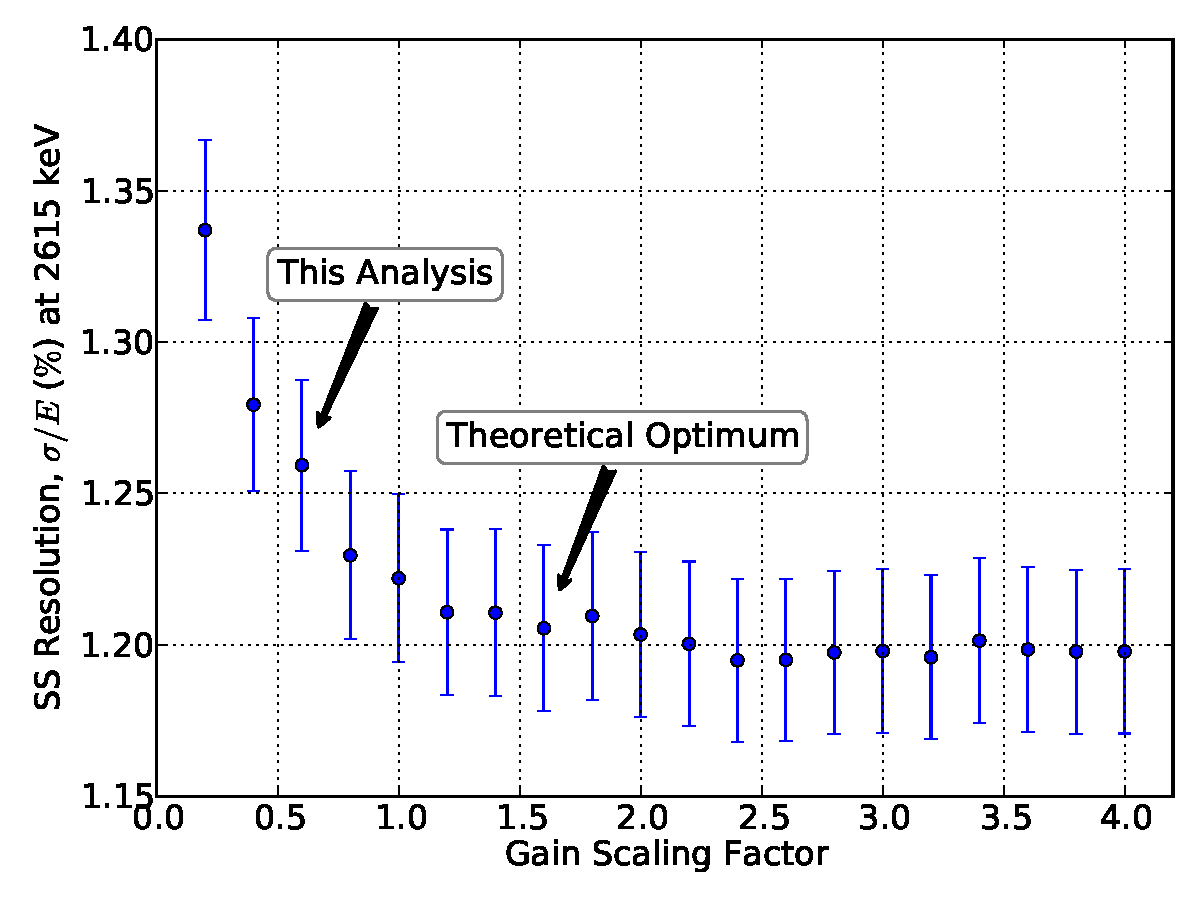
\includegraphics[keepaspectratio=true,width=.49\textwidth]{Denoising_ResVsAPDGain_ss_Run3516.pdf}
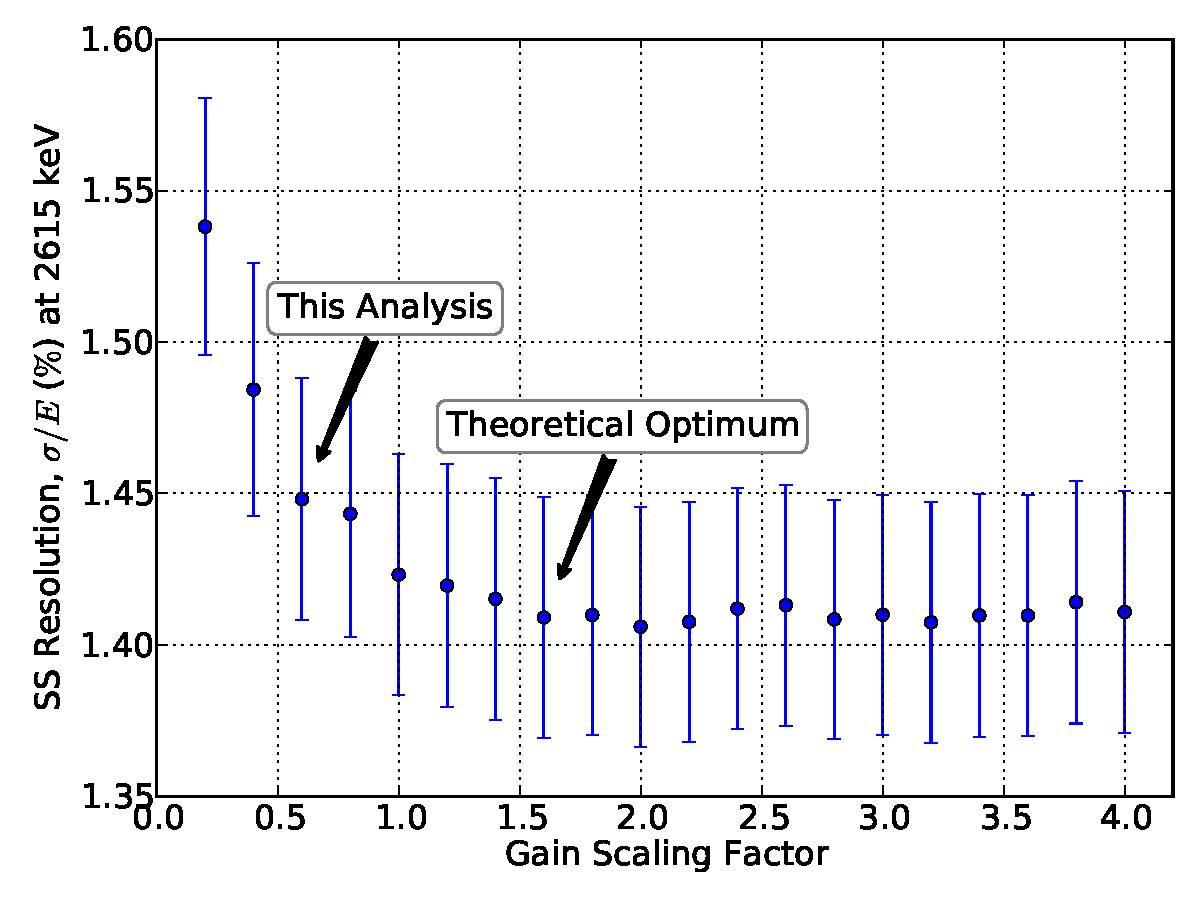
\includegraphics[keepaspectratio=true,width=.49\textwidth]{Denoising_ResVsAPDGain_ss_Run4544.pdf}
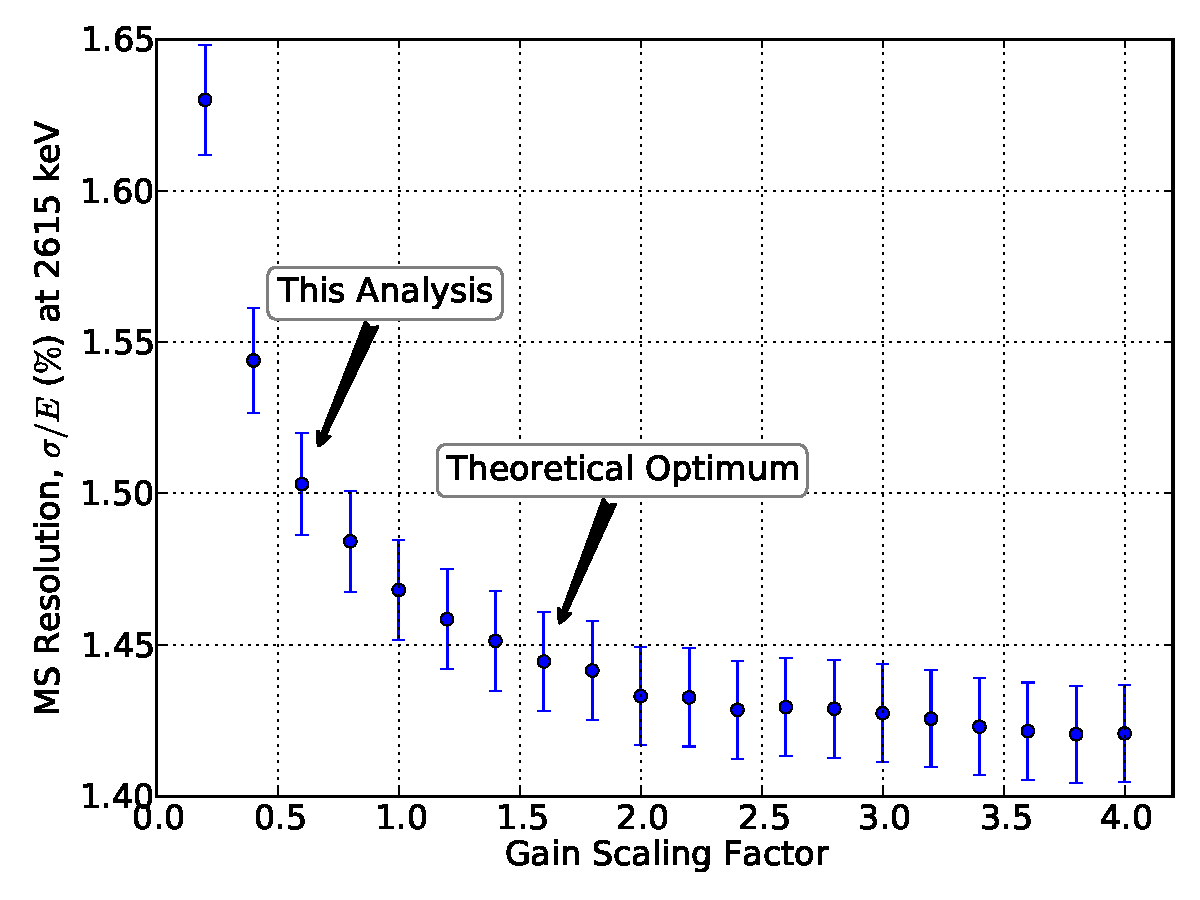
\includegraphics[keepaspectratio=true,width=.49\textwidth]{Denoising_ResVsAPDGain_ms_Run3516.pdf}
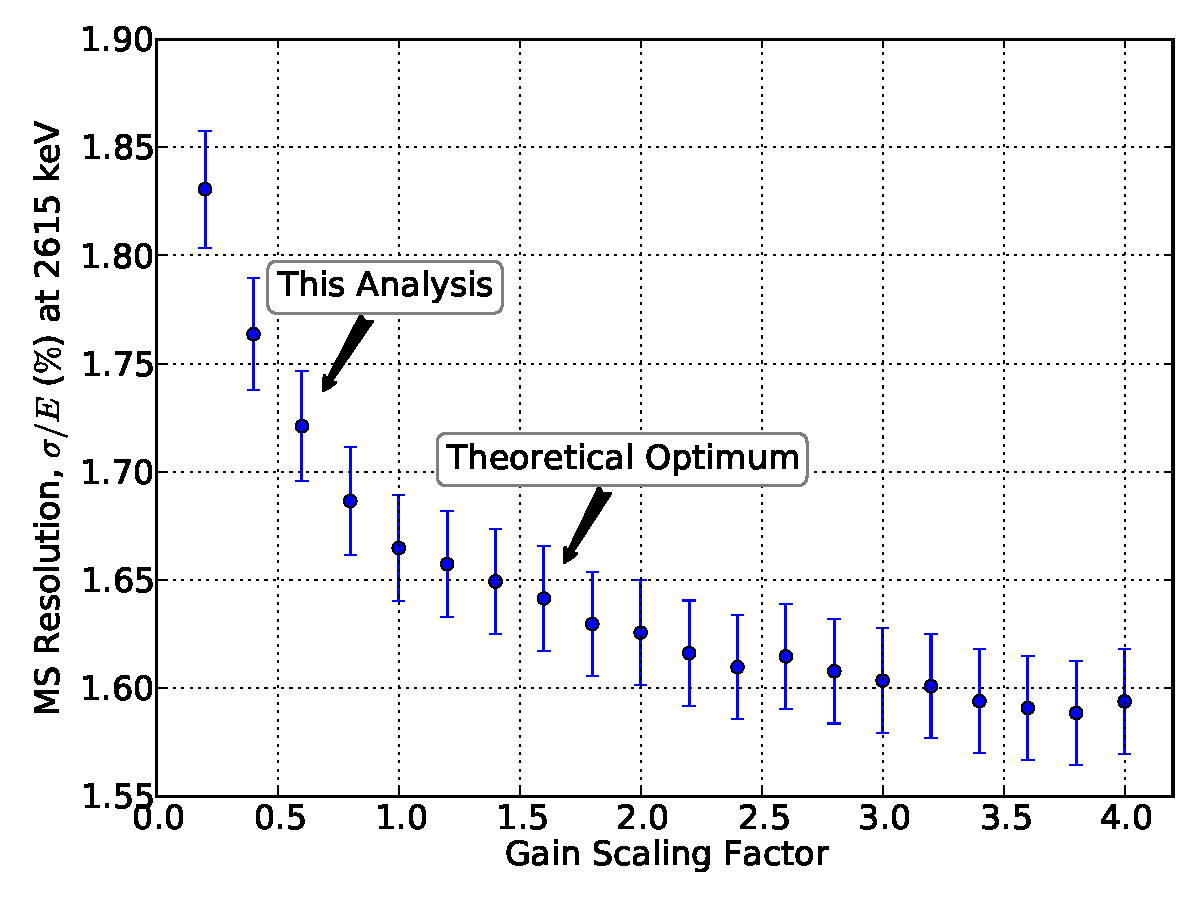
\includegraphics[keepaspectratio=true,width=.49\textwidth]{Denoising_ResVsAPDGain_ms_Run4544.pdf}
\end{center}
\renewcommand{\baselinestretch}{1}
\small\normalsize
\begin{quote}
\caption{It is known that the parameters used for denoising in this analysis are not optimal.  Here we use a scaling factor to adjust the parameter controlling the importance of Poisson noise.  Data from run 3516 and 4544 are shown on the left and right, respectively; top plots show single-site resolution, bottom plots show multi-site resolution.  We can see that an improvement of roughly 0.05 percentage points at 2615 keV could be achieved by moving from the expected optimum.  It is not currently understood why scaling factors above the expected optimum yield further improvements to resolution.}
\label{fig:Denoising_ResVsAPDGain_ScalingFactor}
\end{quote}
\end{figure}
\renewcommand{\baselinestretch}{2}
\small\normalsize

The effect of both of these issues is, loosely speaking, to fool denoising into believing its photon statistics are greater than they truly are; this, in turn, leads it to prefer a higher concentration of signal (more weight on fewer channels) than is ideal.  Thus, the resolution is negatively impacted by these mistakes; the effect of these two issues can be summarized in one scaling factor which controls the importance of Poisson noise.  In figure~\ref{fig:Denoising_ResVsAPDGain_ScalingFactor} sample runs are denoised with different values of this scaling factor, including the value of 0.6 which was used for the present analysis and 1.6 which we would expect to be the optimal choice.  It appears that an improvement in resolution of roughly 0.05 percentage points at 2615 keV will be gained when thes issues are addressed.

However, neither of these mistakes have any impact on the correctness of the constraints.  As a result, the denoised energy measurements should still be unbiased, even if they have worse variance than necessary.  Results from the use of this data will be described in chapter~\ref{ch:DenoisingResults}.

\section{Future Extensions to Denoising}\label{sec:FutureDenoisingExtensions}

As outlined here, denoising is capable of producing optimal estimates of the total energy emitted in scintillation by a particular event; however, it should be noted that this algorithm can be applied to a more general range of problems in the EXO-200 detector with only minor modifications.

\subsection{Anticorrelated Cluster Energies}

One important generalization is in our definition of ``signals.''  In the body of this chapter, we have worked on the assumption that a signal consists of a simultaneous set of energy deposits in the bulk of the detector, possibly at multiple locations.  We do this because it must be possible for denoising to break degeneracies between signals -- by specifying that two different signals must have occurred at different times, we give the algorithm a means to discriminate between light coming from the two different signals and assign energy properly to each of them.

Historically, time was the only useful variable for this sort of discrimination; because multiple APD channels were added together and all APD channels were treated as identical in this sum, a significant amount of information was discarded and there were no remaining parameters to use for signal separation except for the signal time.

However, this denoising algorithm makes use of additional information: the relative magnitudes of each APD gang.  By depending on a highly detailed lightmap, we have incorporated information about which channels should see light most from energy deposits at different positions.   As a result, if we permit two ``signals'' which are simultaneous in time, it should be possible to separate their energy content by comparing their positions to the set of channels which see more light.  This would allow us to produce anti-correlated energy measurements of individual clusters, which should give a significant improvement in the energy resolution achievable for clusters within an event.

In principle, this is entirely feasible -- in the extreme case, when two clusters are at opposite ends of the detector we can expect them to produce light on an entirely different set of channels, and it should be quite easy to separate light produced by each.  However, this extension of our algorithm does present some practical challenges.

In EXO's reconstruction, light signals which are found close together in time are aggressively merged together, ensuring that denoising will never encounter light signals which are very close in time; this assures us that two signals separated in time will be well-separated, and there will not be a near-degeneracy which could render the solver algorithm unstable.

However, charge clusters are merged much less aggressively, and some bugs exist which have minimal effect on the main analysis but permit the existence of clusters very near to each other.  For denoising to separate simultaneous light signals solely based on their relative position, they must be separated far enough that their respective light yields on nearby APD channels are significantly different, which is not at all guaranteed by reconstruction.  As a result, denoising can only fit simultaneous signals separately if it performs a re-clustering process in which clusters occurring near each other are artificially merged together for the purpose of denoising.  The threshold for merging clusters together would require further study, and might be different in each of the three coordinate directions.

Such an analysis would not have a significant impact on single-site data, so it would have minimal impact on our primary goal of searching for double-beta decay.  However, it could have a significant impact on a search for excited-state two-neutrino double-beta decay by improving the resolution of gamma lines associated with Barium de-excitation.  Barabash states in~\cite{Barabash2010} that the dominant mode of excited-state $2\nu \beta\beta$ decay will be to the $0^{+}_1$ state, which in $^{136}Ba$ would lead to the emission of a $760$ keV and $819$ keV gamma in coincidence; if denoising could be accomplished on individual clusters, the sensitivity to these gamma lines could be significantly enhanced.

There are also potential benefits to our understanding of the detector itself.  Currently the only mono-energetic beta calibration available for EXO is the double-escape peak, formed when a gamma particle enters the detector, pair-produces an electron and positron, and the positron interacts with an electron and emits gammas which travel sufficiently far from the initial interaction site so that the initial electron interactions and gamma interactions can be clearly separated.  Currently we have the ability to separate charge yield from gammas and the initial electron in some of these events, allowing us to understand the different charge yields from gammas and betas.  However, we have no similar capabilities for light yield because the gamma and beta interactions are treated as just one ``signal.''  If we could separate the light yield from these spatially separated clusters, we could use these events to understand both the light and charge yield for different types of interactions.

Another type of detector study which might benefit from anticorrelated cluster energies is the Compton telescope.  This is a technique that combines our knowledge of cluster energies and scattering angles, along with the Compton scattering formula~\cite{ComptonScattering}, which allows us to produce estimates of the origin of the incident gamma.  Such a technique permits us to study the sources of our backgrounds, informing future attempts to reduce them by indicating which materials had the most significant negative effect.  The accuracy by which we place the origin of the incident gammas is strongly related to the accuracy of our measurements of the energies of the individual clusters, so it is expected that improving the accuracy of our cluster energies would have a positive impact on our ability to locate the backgrounds of our experiment.

The last benefit to this approach is more technical: evaluating the lightmap for a multi-site event requires an energy-weighted combination of the values of the lightmap at individual cluster locations.  This process is complicated and error-prone, and can be avoided entirely when we treat each signal instead as having a single well-defined position.

\subsection{Wire Denoising}

The current EXO-200 resolution is limited by the scintillation resolution of the APDs.  As a result, little benefit is anticipated from denoising the wires.  However, it is possible that a future detector could reduce the scintillation noise to a point where resolution of the wires is non-negligible; alternatively, a future detector could have noise which is correlated between wires and APDs, making it possible to use noise information from the wires to improve our scintillation resolution even though no direct benefit is expected to the wire resolution itself.

In any case, it is possible to apply equations~\ref{eqn:SystemToSolve} to a system with a combination of wires and APDs without significant adjustment.  The template functions $Y[t]$ will of course be significantly different, and must include a time offset to account for the different time of arrival of the electrons and photons.  The ``lightmap'' of charge will be far less diffuse than for APDs because charge from any location generally drifts directly to only a small number of wires along externally imposed field lines.  And finally, because electron statistics should be negligible and signal amplification should not be a noisy process, for wire channels we would modify equation~\ref{eqn:DefinitionOfQ} to state that $q(i_{wire}, b) = 0$.  In this sense, denoising of wires consists of minimizing the variance in the energy estimator due to electronic noise, and using the wires to improve our denoising of APDs consists of using information about the wires to reduce variance due to electronic noise without expecting any correlations between APD and wire signals, all while ensuring that the energy estimates are unbiased by retaining the same constraints.

\section{Summary}

\textcolor{red}{At least a brief comment on why conventional approaches don't apply here.}
